\documentclass[11pt,compress,t,notes=noshow, xcolor=table]{beamer}

% graphicx and color are loaded via lmu-lecture.sty
% maxwidth is the original width if it is less than linewidth
% otherwise use linewidth (to make sure the graphics do not exceed the margin)
% TODO: Remove once cleared to be superfluous
% \makeatletter
% \def\maxwidth{ %
%   \ifdim\Gin@nat@width>\linewidth
%     \linewidth
%   \else
%     \Gin@nat@width
%   \fi
% }
% \makeatother

% ---------------------------------%
% latex-math dependencies, do not remove:
% - mathtools
% - bm
% - siunitx
% - dsfont
% - xspace
% ---------------------------------%

%--------------------------------------------------------%
%       Language, encoding, typography
%--------------------------------------------------------%

\usepackage[english]{babel}
\usepackage[utf8]{inputenc} % Enables inputting UTF-8 symbols
% Standard AMS suite (loaded via lmu-lecture.sty)

% Font for double-stroke / blackboard letters for sets of numbers (N, R, ...)
% Distribution name is "doublestroke"
% According to https://mirror.physik.tu-berlin.de/pub/CTAN/fonts/doublestroke/dsdoc.pdf
% the "bbm" package does a similar thing and may be superfluous.
% Required for latex-math
\usepackage{dsfont}

% bbm – "Blackboard-style" cm fonts (https://www.ctan.org/pkg/bbm)
% Used to be in common.tex, loaded directly after this file
% Maybe superfluous given dsfont is loaded
% TODO: Check if really unused?
% \usepackage{bbm}

% bm – Access bold symbols in maths mode - https://ctan.org/pkg/bm
% Required for latex-math, preferred over \boldsymbol
% https://tex.stackexchange.com/questions/3238/bm-package-versus-boldsymbol
\usepackage{bm}

% pifont – Access to PostScript standard Symbol and Dingbats fonts
% Used for \newcommand{\xmark}{\ding{55}, which is never used
% aside from lecture_advml/attic/xx-automl/slides.Rnw
% \usepackage{pifont}

% Quotes (inline and display), provdes \enquote
% https://ctan.org/pkg/csquotes
\usepackage{csquotes}

% Adds arg to enumerate env, technically superseded by enumitem according
% to https://ctan.org/pkg/enumerate
% Replace with https://ctan.org/pkg/enumitem ?
% Even better: enumitem is not really compatible with beamer and breaks all sorts of things
% particularly the enumerate environment. The enumerate package also just isn't required
% from what I can tell so... don't re-add it I guess?
% \usepackage{enumerate}

% Line spacing - provides \singlespacing \doublespacing \onehalfspacing
% https://ctan.org/pkg/setspace
% \usepackage{setspace}

% mathtools – Mathematical tools to use with amsmath
% https://ctan.org/pkg/mathtools?lang=en
% latex-math dependency according to latex-math repo
\usepackage{mathtools}

% Maybe not great to use this https://tex.stackexchange.com/a/197/19093
% Use align instead -- TODO: Global search & replace to check, eqnarray is used a lot
% $ rg -f -u "\begin{eqnarray" -l | grep -v attic | awk -F '/' '{print $1}' | sort | uniq -c
%   13 lecture_advml
%   14 lecture_i2ml
%    2 lecture_iml
%   27 lecture_optimization
%   45 lecture_sl
\usepackage{eqnarray}
% For shaded regions / boxes
% Used sometimes in optim
% https://www.ctan.org/pkg/framed
\usepackage{framed}

%--------------------------------------------------------%
%       Cite button (version 2024-05)
%--------------------------------------------------------%

% Superseded by style/ref-buttons.sty, kept just in case these don't work out somehow.

% Note this requires biber to be in $PATH when running,
% telltale error in log would be e.g. Package biblatex Info: ... file 'authoryear.dbx' not found
% aside from obvious "biber: command not found" or similar.
% Tried moving this to lmu-lecture.sty but had issues I didn't quite understood,
% so it's here for now.

\usepackage{hyperref}

% Only try adding a references file if it exists, otherwise
% this would compile error when references.bib is not found
% NOTE: Bibliography packages (usebib, biblatex) are now loaded by ref-buttons.sty when needed
% This keeps all bibliography-related setup in one place

% Legacy \citelink command removed - superseded by ref-buttons.sty

%--------------------------------------------------------%
%       Displaying code and algorithms
%--------------------------------------------------------%

% Reimplements verbatim environments: https://ctan.org/pkg/verbatim
% verbatim used sed at least once in
% supervised-classification/slides-classification-tasks.tex
% Removed since code should not be put on slides anyway
% \usepackage{verbatim}

% Both used together for algorithm typesetting, see also overleaf: https://www.overleaf.com/learn/latex/Algorithms
% algorithmic env is also used, but part of the bundle:
%   "algpseudocode is part of the algorithmicx bundle, it gives you an improved version of algorithmic besides providing some other features"
% According to https://tex.stackexchange.com/questions/229355/algorithm-algorithmic-algorithmicx-algorithm2e-algpseudocode-confused
\usepackage{algorithm}
\usepackage{algpseudocode}

%--------------------------------------------------------%
%       Tables
%--------------------------------------------------------%

% multi-row table cells: https://www.namsu.de/Extra/pakete/Multirow.html
% Provides \multirow
% Used e.g. in evaluation/slides-evaluation-measures-classification.tex
\usepackage{multirow}

% colortbl: https://ctan.org/pkg/colortbl
% "The package allows rows and columns to be coloured, and even individual cells." well.
% Provides \columncolor and \rowcolor
% \rowcolor is used multiple times, e.g. in knn/slides-knn.tex
\usepackage{colortbl}

% long/multi-page tables: https://texdoc.org/serve/longtable.pdf/0
% Not used in slides
% \usepackage{longtable}

% pretty table env: https://ctan.org/pkg/booktabs
% Is used
% Defines \toprule
\usepackage{booktabs}

%--------------------------------------------------------%
%       Figures: Creating, placing, verbing
%--------------------------------------------------------%

% wrapfig - Wrapping text around figures https://de.overleaf.com/learn/latex/Wrapping_text_around_figures
% Provides wrapfigure environment -used in lecture_optimization
\usepackage{wrapfig}

% Sub figures in figures and tables
% https://ctan.org/pkg/subfig -- supersedes subfigure package
% Provides \subfigure
% \subfigure not used in slides but slides-tuning-practical.pdf errors without this pkg, error due to \captionsetup undefined
\usepackage{subfig}

% Actually it's pronounced PGF https://en.wikibooks.org/wiki/LaTeX/PGF/TikZ
\usepackage{tikz}

% No idea what/why these settings are what they are but I assume they're there on purpose
\usetikzlibrary{shapes,arrows,automata,positioning,calc,chains,trees, shadows}
\tikzset{
  %Define standard arrow tip
  >=stealth',
  %Define style for boxes
  punkt/.style={
    rectangle,
    rounded corners,
    draw=black, very thick,
    text width=6.5em,
    minimum height=2em,
    text centered},
  % Define arrow style
  pil/.style={
    ->,
    thick,
    shorten <=2pt,
    shorten >=2pt,}
}

\tikzstyle{squ}=[draw, rectangle, minimum size = 5mm]
\tikzstyle{del}=[squ, fill = white]
\tikzstyle{vec}=[draw, rectangle, fill = white, minimum width=5mm, minimum height=1cm, inner sep = 2pt]

% textpos package to allow absolute placement of environments like figures
% See e.g. https://datumorphism.leima.is/til/programming/latex-beamer-textblock-position/
%  - absolute: Enables absolute positioning mode where coordinates are measured from the top-left corner of the page/frame, rather than relative to the current text position.
%  - overlay: Makes the positioned content behave as an overlay that doesn't affect the normal text flow or spacing. Without this, positioned elements could interfere with the document's layout.
% 
%   The \textblock* environment creates a text block at absolute coordinates:
% 
%   \begin{textblock*}{\linewidth}(0cm,4cm) % (x,y) from top-left of frame
%     \imageC[1]{figure/cov_funs/cov_matern.pdf}
%   \end{textblock*}
\usepackage[absolute,overlay]{textpos}

%--------------------------------------------------------%
%       Beamer setup and custom macros & environments
%--------------------------------------------------------%

% Main sty file for beamer setup (layout, style, lecture page numbering, etc.)
% For long-term maintenance, this may me refactored into a more modular set of .sty files
\usepackage{../../style/lmu-lecture-new}
% Custom itemize wrappers, itemizeS, itemizeL, etc

% Used regularly
\let\code=\texttt

% Not sure what/why this does
\setkeys{Gin}{width=0.9\textwidth}

% -- knitr leftovers --
% These may be used by knitr/R Markdown workflows in other lectures
\makeatletter
\def\maxwidth{ %
  \ifdim\Gin@nat@width>\linewidth
    \linewidth
  \else
    \Gin@nat@width
  \fi
}
\makeatother

% Define colors for syntax highlighting (may be used by knitr)
\definecolor{fgcolor}{rgb}{0.345, 0.345, 0.345}
\definecolor{shadecolor}{rgb}{.97, .97, .97}

% knitr code output environment
\newenvironment{knitrout}{}{}

\newcommand{\citebutton}[2]{%
\beamergotobutton{\href{#2}{#1}}%
}

\newcommand{\ques}{\textbf{\textcolor{red}{Question:  }}}
\newcommand{\questionssofar}{\begin{frame}\frametitle{Any questions?}\end{frame}}

\definecolor{texblue}{rgb}{0, 0, 1}
\def\myblue#1{\textcolor{texblue}{#1}}
\newcommand{\blu}[1]{\textcolor{blue}{#1}}
\newcommand{\org}[1]{\textcolor{orange}{#1}}

\def\rmA{{\mathbf{A}}}
\def\rmE{{\mathbf{E}}}
\def\rmR{{\mathbf{R}}}
\def\rmU{{\mathbf{U}}}
\def\rmW{{\mathbf{W}}}

\newcommand\warning{%
 \makebox[1.4em][c]{%
 \makebox[0pt][c]{\raisebox{.1em}{\scriptsize!}}%
 \makebox[0pt][c]{\color{red}\normalsize$\bigtriangleup$}}}%

% Can't find a reason why common.tex is not just part of this file?
\input{../../style/common_new}


% custom packages
\usepackage{subfig}
\usepackage{psfrag}
\usepackage{algorithm}
\usepackage{algpseudocode}
\usepackage{eqnarray}
\usepackage{arydshln}
\usepackage{tabularx}
\usepackage{placeins}
\usepackage{tikz}
\usepackage{setspace}
\usepackage{colortbl}
\usepackage{mathtools}
\usepackage{wrapfig}
\usepackage{listings}

\usepackage{framed}
\makeatletter
\newenvironment{kframe}{%
 \def\at@end@of@kframe{}%
 \ifinner\ifhmode%
  \def\at@end@of@kframe{\end{minipage}}%
  \begin{minipage}{\columnwidth}%
 \fi\fi%
 \def\FrameCommand##1{\hskip\@totalleftmargin \hskip-\fboxsep
 \colorbox{shadecolor}{##1}\hskip-\fboxsep
     % There is no \\@totalrightmargin, so:
     \hskip-\linewidth \hskip-\@totalleftmargin \hskip\columnwidth}%
 \MakeFramed {\advance\hsize-\width
   \@totalleftmargin\z@ \linewidth\hsize
   \@setminipage}}%
 {\par\unskip\endMakeFramed%
 \at@end@of@kframe}
\makeatother

%-------------------------
% Q&A Slides
%-------------------------

\usepackage{etoolbox}
\usepackage{pdftexcmds}

\newlength{\qabuttonheight}   \setlength{\qabuttonheight}{1.4em}
\newcommand{\qaframecolor}{gray}     % colour of the button frame
\newcommand{\qaroundness}{4pt}
\newcommand{\qalinewidth}{0.8pt}

\makeatletter
\newcommand{\qalist}{}
\newsavebox{\qa@measure}

% rounded, transparent button; fits the text, wraps if too long
\newcommand{\qa@box}[2]{%
  \savebox{\qa@measure}{#2}%
  \hyperlink{#1}{%
    \begin{tikzpicture}[baseline=(qa@n.base)]
      \ifdim\wd\qa@measure>\dimexpr\linewidth-12pt-2\qalinewidth\relax
        \node[draw=\qaframecolor, line width=\qalinewidth,
              rounded corners=\qaroundness, inner xsep=6pt, inner ysep=2pt,
              minimum height=\qabuttonheight,
              text width=\dimexpr\linewidth-12pt-2\qalinewidth\relax,
              align=left, text=normal text.fg] (qa@n) {#2};
      \else
        \node[draw=\qaframecolor, line width=\qalinewidth,
              rounded corners=\qaroundness, inner xsep=6pt, inner ysep=2pt,
              minimum height=\qabuttonheight,
              text=normal text.fg] (qa@n) {#2};
      \fi
    \end{tikzpicture}}}

% small "Back" button
\newcommand{\qa@backbtn}[1]{%
  \hyperlink{#1}{%
    \begin{tikzpicture}[baseline=(b.base)]
      \node[draw=\qaframecolor, line width=\qalinewidth,
            rounded corners=\qaroundness, inner xsep=6pt, inner ysep=2pt,
            text=normal text.fg] (b) {\footnotesize Back};
    \end{tikzpicture}}}

% one entry on the answer slides: {key}{question}{answer}
\newcommand{\qa@entry}[3]{%
  \hypertarget{#1}{}%
  {\color{red}\textbf{Question:}}~#2\par
  \smallskip
  \textbf{Answer:}~#3\par
  \nopagebreak\smallskip
  \noindent\hfill\qa@backbtn{#1-src}\par
  \bigskip
}

% \qa{question}{answer}
\newcommand{\qa}[2]{%
  \begingroup
  \edef\qa@key{qa:\pdf@mdfivesum{\detokenize{#1}}}%
  \ifcsname \qa@key @seen\endcsname\else
    \global\expandafter\let\csname \qa@key @seen\endcsname\relax
    \edef\qa@tmp{\noexpand\qa@entry{\qa@key}}%
    \expandafter\gappto\expandafter\qalist\expandafter{\qa@tmp{#1}{#2}}%
  \fi
  \par\smallskip\noindent
  \hypertarget{\qa@key -src}{}%
  \qa@box{\qa@key}{{\color{red}\textbf{Question:}}~#1}%
  \endgroup
}
\makeatother

% all answers, broken over as many slides as needed
\newcommand{\qaslides}{%
  \begin{frame}[allowframebreaks,noframenumbering,plain]{Backup: Questions \& Answers}
    \qalist
  \end{frame}}
\usepackage{tcolorbox}
\usepackage{dsfont}
\usepackage{tikz}
\usetikzlibrary{decorations.pathreplacing}


% Run bibliography entries together instead of breaking after each block
\setbeamertemplate{bibliography entry title}{}
\setbeamertemplate{bibliography entry location}{}
\setbeamertemplate{bibliography entry note}{}

% Numbered labels [1], [2] instead of the little paper icon
\setbeamertemplate{bibliography item}{\insertbiblabel}

% ToC
\AtBeginSection[]{
	\begin{frame}[noframenumbering, plain]
	\frametitle{Outline}
	\setcounter{tocdepth}{1}
	\tableofcontents[currentsection]
\end{frame}
}



\newcommand{\paperfigure}[4][0.3\textheight]{%
  \IfFileExists{#3}{\includegraphics[width=#2]{#3}}{%
    \tikz\node[draw=gray!60, dashed, fill=gray!6, rounded corners=2pt,
               minimum width=#2, minimum height=#1, text width=0.9*#2,
               align=center, font=\scriptsize, text=gray!70!black]
      {\textbf{PAPER FIGURE}\\[2pt] #4\\[2pt] \texttt{\detokenize{#3}}};}}

% Attention masks: one cell per (query \qq, key \kk) pair, queries top to
% bottom. The last argument is a pgfmath expression in \qq and \kk returning
% a color code: 0 = not computed, 1 = teal, 2 = violet, 3 = orange.
% Usage: \attnmask{x offset}{n}{cell size}{expression}
\newcommand{\attnmask}[4]{%
  \foreach \qq in {1,...,#2}{
    \foreach \kk in {1,...,#2}{
      \pgfmathtruncatemacro{\mcode}{#4}
      \ifcase\mcode \def\mcol{gray!8}\or \def\mcol{teal!50}\or \def\mcol{violet!45}\or \def\mcol{orange!55}\fi
      \filldraw[fill=\mcol, draw=white, line width=0.3pt]
        ({#1 + (\kk - 1) * #3}, {(#2 - \qq) * #3}) rectangle ++(#3, #3);
    }
  }
}

% Good / bad entries in comparison tables
\newcommand{\good}[1]{\textcolor{teal!60!black}{#1}}
\newcommand{\bad}[1]{\textcolor{red!70!black}{#1}}




\title{Deep Learning for NLP II}

\begin{document}

\titlemeta{
Linear RNNs and State Space Models
}{}{
figure/mamba.png
}{
\item Efficient attention variants
\item Introduction to linear RNNs
\item Overview of Mamba
}

% ------------------------------------------------------------------------------



\begin{frame}{Recap: Is Attention All You Need?}
\vfill
\begin{itemize}
\item We have discussed several methods to modify LMs: RAGs, MDLMs, MoEs, LMs with latent tokenization
\item However, they all keep one aspect of the LM architecture unchanged: attention
\end{itemize}

\medskip
\medskip
\medskip

\centering
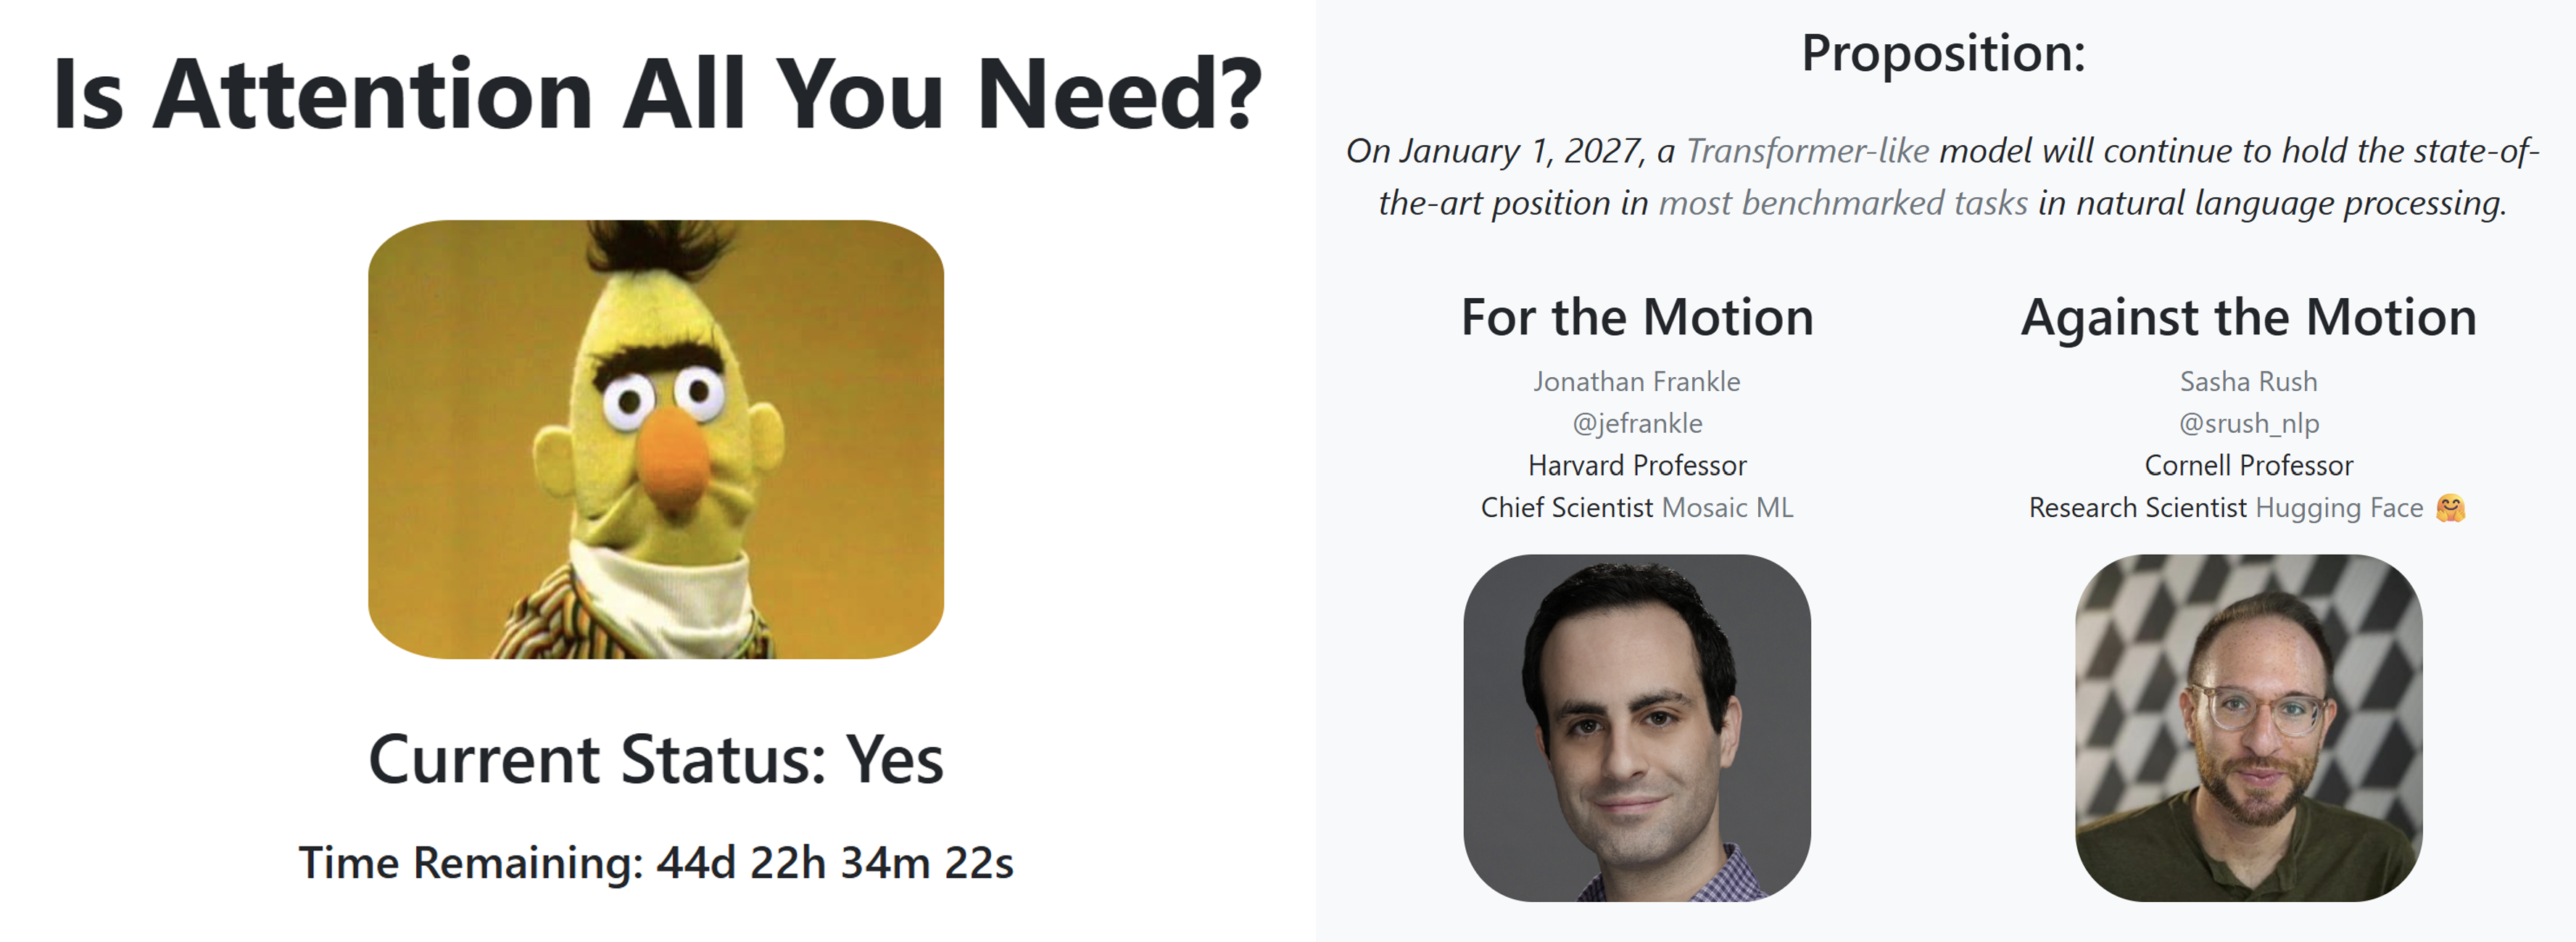
\includegraphics[width=0.9\textwidth]{figure/bet_combined.png}\\
\url{https://www.isattentionallyouneed.com/}
  
\vfill
\end{frame}




\begin{frame}{Recap: Parameters Vs.\ Compute}
\vfill
\begin{itemize}
\item Embeddings and FFNs hold most of the \textbf{parameters} in LMs
\item Attention holds fewer parameters, but its \textbf{compute} grows with $n^2$
\item Example: at 16K tokens, attention accounts for over 80\,\% of all transformer operations ($d_{model} = 768$)
\end{itemize}

\medskip
\medskip

\centering
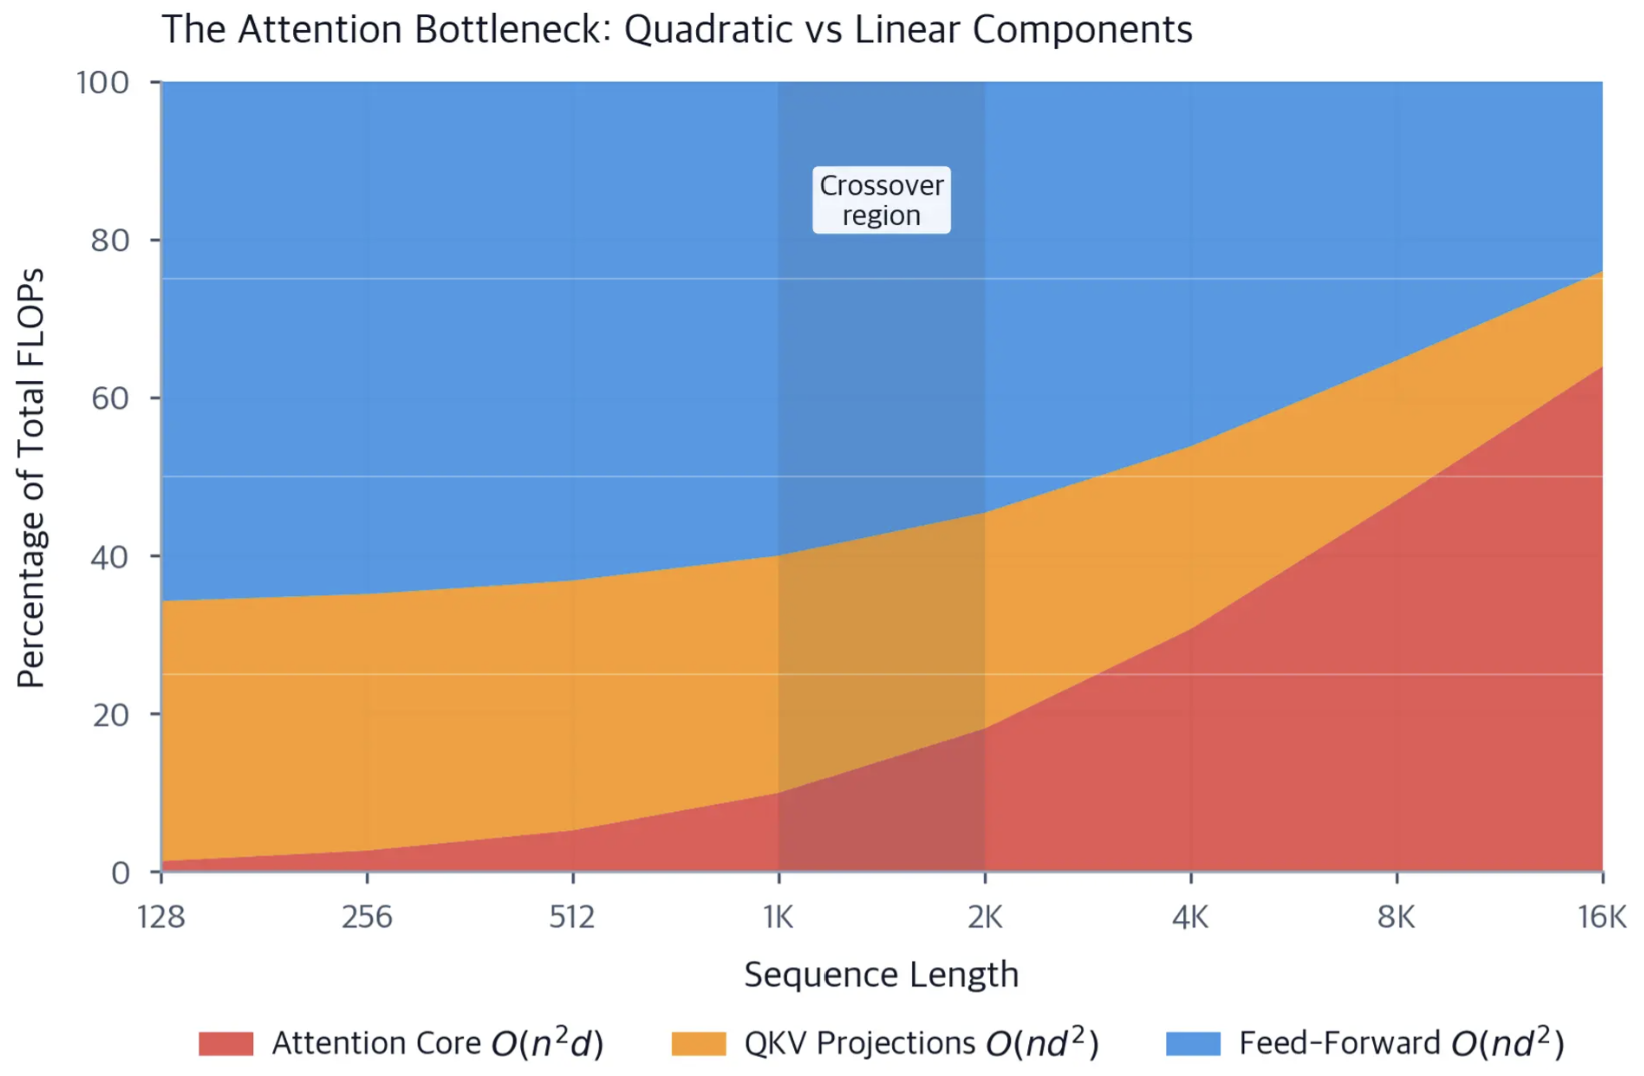
\includegraphics[width=0.7\textwidth]{figure/compute_att.png}\\
  
\vfill
\end{frame}




\begin{frame}{Recap: Self-Attention Is Quadratic}

\vfill

\begin{itemize}
  \item Every token attends to every earlier token, so we need to compute c.\ $n^2/2$ scores per head and layer
  \item Doubling the context roughly quadruples the attention compute
  \item FlashAttention also does not help here (why?)
\end{itemize}

\medskip
\medskip


\begin{center}
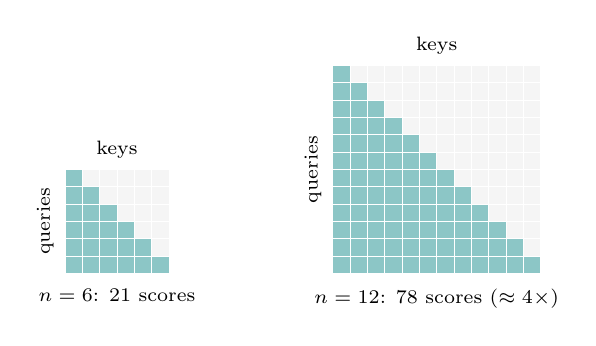
\begin{tikzpicture}[font=\scriptsize]
  \def\cs{0.22}
  \foreach \n/\ox/\lab in {6/0/{$n = 6$: 21 scores}, 12/3.4/{$n = 12$: 78 scores ($\approx 4\times$)}}{
    \foreach \qq in {1,...,\n}{
      \foreach \kk in {1,...,\n}{
        \ifnum\kk>\qq
          \def\mcol{gray!8}
        \else
          \def\mcol{teal!45}
        \fi
        \filldraw[fill=\mcol, draw=white, line width=0.3pt]
          ({\ox + (\kk - 1) * \cs}, {(\n - \qq) * \cs}) rectangle ++(\cs, \cs);
      }
    }
    \node[anchor=north] at ({\ox + \n * \cs / 2}, -0.08) {\lab};
    \node[anchor=south] at ({\ox + \n * \cs / 2}, {\n * \cs + 0.02}) {keys};
    \node[anchor=south, rotate=90] at ({\ox - 0.02}, {\n * \cs / 2}) {queries};
  }
\end{tikzpicture}
\end{center}


\vfill

\end{frame}



\begin{frame}
\vfill
\medskip
\medskip
\centering\LARGE\bfseries Can we make attention cheaper by attending to fewer tokens?
\vfill
\end{frame}



\begin{frame}{Outline}
\tableofcontents
\end{frame}


\section{Efficient Attention Variants}


\begin{frame}{Sparse Attention}

\vfill

\begin{itemize}
  \item Compute only a subset of the $n^2$ scores: each token attends to $w \ll n$ other tokens $\rightarrow$ $O(n w)$
  \item Common strategy: \textbf{sliding window} around each token
\end{itemize}

\medskip
\medskip


\begin{center}
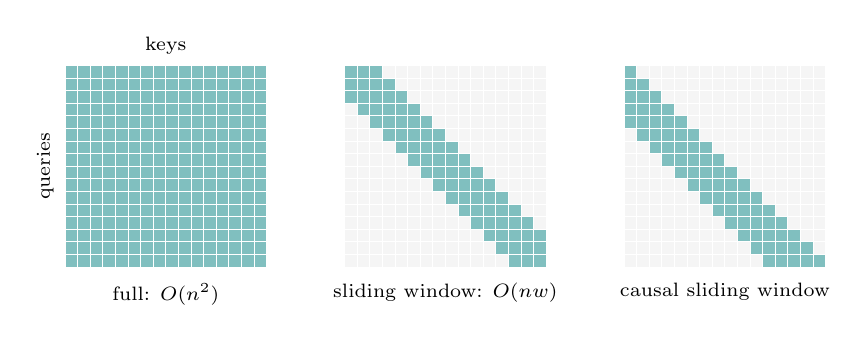
\begin{tikzpicture}[font=\scriptsize]
  \def\cs{0.16}
  \attnmask{0}{16}{\cs}{1}
  \attnmask{3.55}{16}{\cs}{(abs(\qq - \kk) <= 2) ? 1 : 0}
  \attnmask{7.1}{16}{\cs}{(\kk <= \qq && \qq - \kk <= 4) ? 1 : 0}
  \node[anchor=north] at (1.28, -0.08) {full: $O(n^2)$};
  \node[anchor=north] at (4.83, -0.08) {sliding window: $O(n w)$};
  \node[anchor=north] at (8.38, -0.08) {causal sliding window};
  \node[anchor=south] at (1.28, 2.58) {keys};
  \node[anchor=south, rotate=90] at (-0.02, 1.28) {queries};
\end{tikzpicture}
\end{center}


\vfill

\end{frame}



\begin{frame}{Effect of Sliding Windows}


\vfill

\begin{itemize}
\item Stacking layers spreads information further (cf.\ \textbf{receptive fields} in CNNs and GNNs)
  \item With window $w$, information moves up to $w$ positions per layer $\rightarrow$ up to $L \cdot w$ after $L$ layers
  \item This is also called \textbf{local attention}
\end{itemize}

\medskip
\medskip


\begin{center}
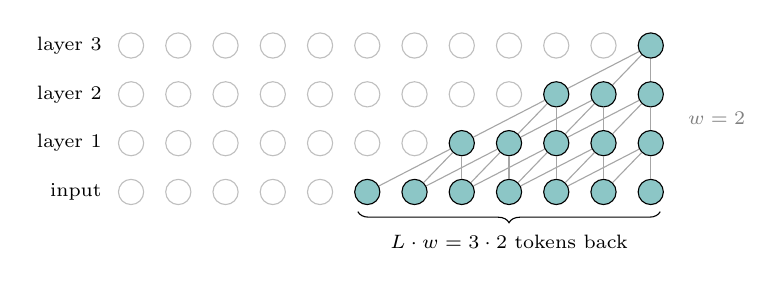
\begin{tikzpicture}[font=\scriptsize, nd/.style={circle, draw, inner sep=0pt, minimum size=3.2mm}]
  \def\dx{0.6} \def\dy{0.62} \def\ww{2}
  % nodes; teal = in the receptive field of the last token in the top layer
  \foreach \lay in {0,...,3}{
    \pgfmathtruncatemacro{\lo}{12 - (3 - \lay) * \ww}
    \foreach \p in {1,...,12}{
      \ifnum\p<\lo
        \node[nd, fill=white, draw=gray!50] (n\lay-\p) at ({\p * \dx}, {\lay * \dy}) {};
      \else
        \node[nd, fill=teal!45] (n\lay-\p) at ({\p * \dx}, {\lay * \dy}) {};
      \fi
    }
  }
  % edges inside the cone
  \foreach \lay in {1,...,3}{
    \pgfmathtruncatemacro{\pl}{\lay - 1}
    \pgfmathtruncatemacro{\lo}{12 - (3 - \lay) * \ww}
    \foreach \p in {\lo,...,12}{
      \foreach \off in {0,...,\ww}{
        \pgfmathtruncatemacro{\src}{\p - \off}
        \draw[gray!70] (n\pl-\src) -- (n\lay-\p);
      }
    }
  }
  \foreach \lay/\lab in {0/input, 1/layer 1, 2/layer 2, 3/layer 3}{
    \node[anchor=east] at (0.35, {\lay * \dy}) {\lab};
  }
  \draw[decorate, decoration={brace, amplitude=4pt, mirror}] ({6 * \dx - 0.12}, -0.25) -- ({12 * \dx + 0.12}, -0.25)
    node[midway, below=5pt] {$L \cdot w = 3 \cdot 2$ tokens back};
  \node[anchor=west, gray, align=left] at ({12 * \dx + 0.35}, {1.5 * \dy}) {$w = 2$};
\end{tikzpicture}
\end{center}

\vfill

\end{frame}


\begin{frame}{Sparse Transformer}

\vfill

\begin{itemize}
  \item \textbf{Factorized attention}: split the attention pattern across two cheap heads \citebutton{Child et al. (2019) \cite{child2019sparse}}{https://arxiv.org/abs/1904.10509}
  \item \textbf{Strided}: previous $\ell$ positions + every $\ell$-th position (images)
  \item \textbf{Fixed}: own block + summary positions at block ends (text)
  \item Any position is reachable in two hops (how?)
\end{itemize}

\medskip
\medskip

\begin{center}
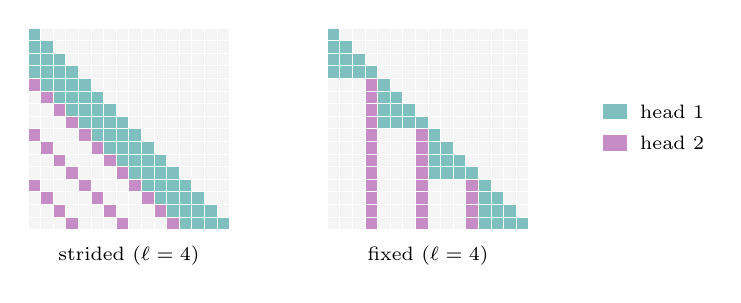
\begin{tikzpicture}[font=\scriptsize]
  \def\cs{0.16}
  % l = 4
  \attnmask{0}{16}{\cs}{(\kk > \qq) ? 0 : ((\qq - \kk < 4) ? 1 : ((mod(\qq - \kk, 4) == 0) ? 2 : 0))}
  \attnmask{3.8}{16}{\cs}{(\kk > \qq) ? 0 : ((floor((\kk - 1) / 4) == floor((\qq - 1) / 4)) ? 1 : ((mod(\kk, 4) == 0) ? 2 : 0))}
  \node[anchor=north] at (1.28, -0.08) {strided ($\ell = 4$)};
  \node[anchor=north] at (5.08, -0.08) {fixed ($\ell = 4$)};
  % legend
  \fill[teal!50] (7.3, 1.4) rectangle ++(0.3, 0.2);
  \node[anchor=west] at (7.65, 1.5) {head 1};
  \fill[violet!45] (7.3, 1.0) rectangle ++(0.3, 0.2);
  \node[anchor=west] at (7.65, 1.1) {head 2};
\end{tikzpicture}
\end{center}


\vfill

\end{frame}



\begin{frame}{Longformer}

\vfill

\begin{itemize}
  \item \textbf{Sliding window} of $w$ tokens in every layer \citebutton{Beltagy et al. (2020) \cite{beltagy2020longformer}}{https://arxiv.org/abs/2004.05150}
  \item \textbf{Dilated} windows in some heads: wider reach at the same cost
  \item \textbf{Global attention} for task tokens (e.g., [CLS], question tokens): they see all tokens, all tokens see them
\end{itemize}

\medskip
\medskip


\begin{center}
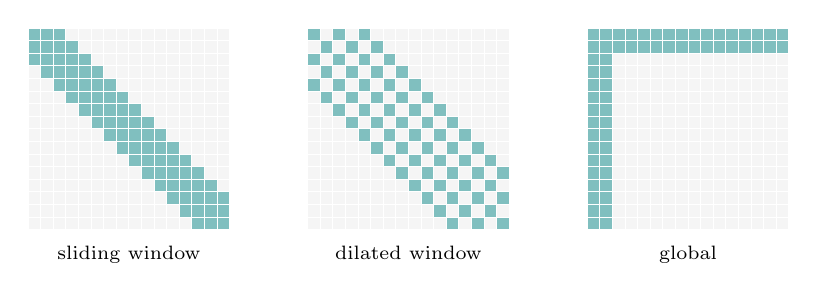
\begin{tikzpicture}[font=\scriptsize]
  \def\cs{0.16}
  \attnmask{0}{16}{\cs}{(abs(\qq - \kk) <= 2) ? 1 : 0}
  \attnmask{3.55}{16}{\cs}{(abs(\qq - \kk) <= 4 && mod(abs(\qq - \kk), 2) == 0) ? 1 : 0}
  \attnmask{7.1}{16}{\cs}{(\qq <= 2 || \kk <= 2) ? 1 : 0}
  \node[anchor=north] at (1.28, -0.08) {sliding window};
  \node[anchor=north] at (4.83, -0.08) {dilated window};
  \node[anchor=north] at (8.38, -0.08) {global};
\end{tikzpicture}
\end{center}

\vfill

\end{frame}



\begin{frame}{BigBird}

\vfill

\begin{itemize}
  \item Combines \textbf{random}, \textbf{window} and \textbf{global} attention \citebutton{Zaheer et al. (2020) \cite{zaheer2020bigbird}}{https://arxiv.org/abs/2007.14062}
  \item Graph view: random edges keep paths between any two tokens short (why not use the global token for this instead?)
\end{itemize}

\medskip
\medskip

\begin{center}
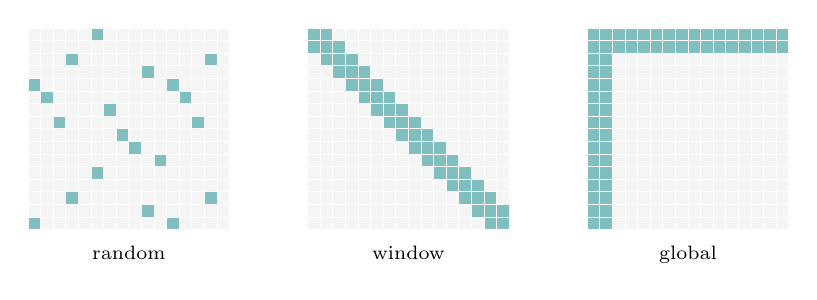
\begin{tikzpicture}[font=\scriptsize]
  \def\cs{0.16}
  \def\rnd{mod(\qq * 7 + \kk * 5 + \qq * \kk * 3, 11) == 0}
  \attnmask{0}{16}{\cs}{(\rnd) ? 1 : 0}
  \attnmask{3.55}{16}{\cs}{(abs(\qq - \kk) <= 1) ? 1 : 0}
  \attnmask{7.1}{16}{\cs}{(\qq <= 2 || \kk <= 2) ? 1 : 0}
  \node[anchor=north] at (1.28, -0.08) {random};
  \node[anchor=north] at (4.83, -0.08) {window};
  \node[anchor=north] at (8.38, -0.08) {global};
\end{tikzpicture}
\end{center}


\vfill

\end{frame}


\begin{frame}{Efficient Attention In Current LMs}

\vfill

\begin{itemize}
  \item No variant clearly beats full attention in performance
  \item Sparsity is GPU-unfriendly
  \item What survived: sliding windows, mixed with global layers
\end{itemize}

\medskip
\medskip


\begin{center}
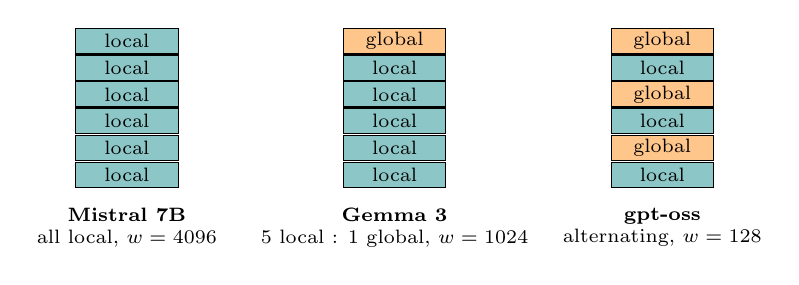
\begin{tikzpicture}[
    font=\scriptsize,
    cell/.style={draw, minimum width=1.3cm, minimum height=3.2mm, inner sep=0pt},
    loc/.style={cell, fill=teal!45},
    glob/.style={cell, fill=orange!45},
  ]
  % layers stacked bottom to top
  \foreach \col/\pattern/\title/\note in {
      0/{0,0,0,0,0,0}/{Mistral 7B}/{all local, $w = 4096$},
      3.4/{0,0,0,0,0,1}/{Gemma 3}/{5 local : 1 global, $w = 1024$},
      6.8/{0,1,0,1,0,1}/{gpt-oss}/{alternating, $w = 128$}%
  }{
    \foreach \m [count=\l] in \pattern {
      \ifnum\m=1
        \node[glob] at (\col, {(\l - 1) * 0.34}) {global};
      \else
        \node[loc] at (\col, {(\l - 1) * 0.34}) {local};
      \fi
    }
    \node[anchor=north, align=center] at (\col, -0.3) {\textbf{\title}\\ \note};
  }
\end{tikzpicture}
\end{center}

\vfill

\end{frame}





\section{Linear RNNs}


\begin{frame}{Recap: Recurrent Neural Networks}

\vfill

\begin{itemize}
  \item Process one token at a time, updating a \textbf{hidden state} $\vec h_t \in \mathbb{R}^N$:
        \[ \vec h_t = f\big(\vec W \vec h_{t-1} + \vec U \vec x_t + \vec b\big) \]
  \item The state summarizes the whole prefix $\vec x_1, \ldots, \vec x_t$
  \item Same parameters at every step, and the state has a fixed size, however long the sequence
\end{itemize}

\medskip
\medskip


\begin{center}
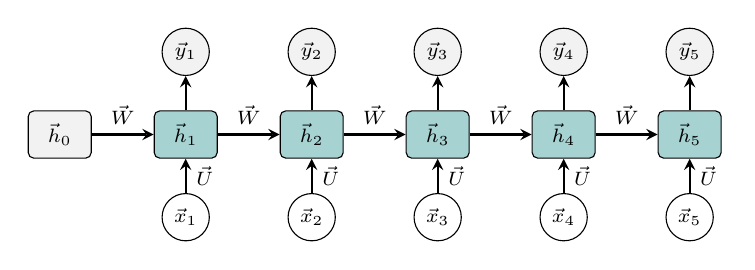
\begin{tikzpicture}[
    font=\scriptsize,
    st/.style={draw, rounded corners=2pt, fill=teal!35, minimum width=8mm, minimum height=6mm},
    io/.style={draw, circle, inner sep=1pt, minimum size=6mm, fill=white},
    flow/.style={->, >=stealth, thick},
  ]
  \node[st, fill=gray!10] (h0) at (0, 0) {$\vec h_0$};
  \foreach \p in {1,...,5}{
    \node[st] (h\p) at ({1.6 * \p}, 0) {$\vec h_{\p}$};
    \node[io] (x\p) at ({1.6 * \p}, -1.05) {$\vec x_{\p}$};
    \node[io, fill=gray!10] (y\p) at ({1.6 * \p}, 1.05) {$\vec y_{\p}$};
    \draw[flow] (x\p) -- node[right] {$\vec U$} (h\p);
    \draw[flow] (h\p) -- (y\p);
  }
  \foreach \p [remember=\p as \pp (initially 0)] in {1,...,5}{
    \draw[flow] (h\pp) -- node[above] {$\vec W$} (h\p);
  }
\end{tikzpicture}
\end{center}

\vfill

\end{frame}

% ------------------------------------------------------------------------------

\begin{frame}{Transformers vs.\ RNNs}

\vfill

\begin{itemize}
  \item RNNs: constant cost per generated token and constant memory
  \item Transformers: cost and memory per token grow with $n$
  \item Advantage of transformers: parallel training
\end{itemize}

\medskip
\medskip


\begin{center}
\small
\begin{tabular}{@{}lcc@{}}
  \toprule
                                      & Transformer               & RNN \\
  \midrule
  Training: parallel over positions   & \good{yes}                & \bad{no} \\
  Training: compute for $n$ tokens    & \bad{$O(n^2)$}            & \good{$O(n)$} \\
  Inference: compute per new token    & \bad{$O(n)$}              & \good{$O(1)$} \\
  Inference: memory                   & \bad{$O(n)$}  & \good{$O(1)$} \\
  \bottomrule
\end{tabular}
\end{center}

\medskip
\medskip

\pause

\begin{center}
\textbf{Can we have parallel training \emph{and} constant-cost inference?}
\end{center}

\vfill

\end{frame}

% ------------------------------------------------------------------------------

\begin{frame}{Challenge 1: Sequential Training}

\vfill

\begin{itemize}
  \item $\vec h_t$ depends on $\vec h_{t-1}$ through the non-linearity $f$ $\rightarrow$ $n$ steps that must run one after another
  \item Each step is a small matrix-vector product, but GPUs are built for large matrix-matrix products
  \item Transformer training processes all $n$ positions at once (causal attention mask + teacher forcing)
\end{itemize}

\vfill

\begin{center}
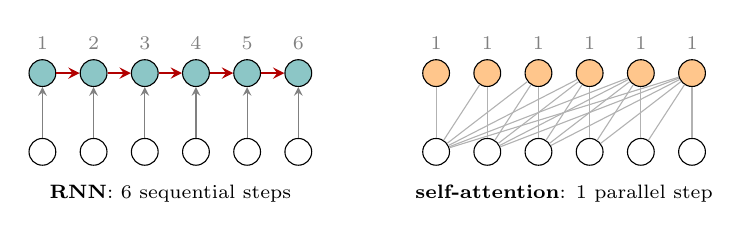
\begin{tikzpicture}[
    font=\scriptsize,
    nd/.style={circle, draw, inner sep=0pt, minimum size=3.4mm},
    flow/.style={->, >=stealth},
  ]
  % ---- RNN: a chain of dependencies -----------------------------------------------
  \foreach \p in {1,...,6}{
    \node[nd] (rx\p) at ({(\p - 1) * 0.65}, 0) {};
    \node[nd, fill=teal!45] (rh\p) at ({(\p - 1) * 0.65}, 1.0) {};
    \draw[flow, gray] (rx\p) -- (rh\p);
    \node[anchor=south, gray] at (rh\p.north) {\p};
  }
  \foreach \p [remember=\p as \pp (initially 1)] in {2,...,6}{
    \draw[flow, thick, red!70!black] (rh\pp) -- (rh\p);
  }
  \node[anchor=north, align=center] at (1.625, -0.3) {\textbf{RNN}: 6 sequential steps};
  % ---- self-attention: everything at once --------------------------------------------
  \foreach \p in {1,...,6}{
    \node[nd] (tx\p) at ({5.0 + (\p - 1) * 0.65}, 0) {};
    \node[nd, fill=orange!45] (th\p) at ({5.0 + (\p - 1) * 0.65}, 1.0) {};
    \node[anchor=south, gray] at (th\p.north) {1};
  }
  \foreach \p in {1,...,6}{
    \foreach \s in {1,...,\p}{
      \draw[gray!60] (tx\s) -- (th\p);
    }
  }
  \node[anchor=north, align=center] at (6.625, -0.3) {\textbf{self-attention}: 1 parallel step};
\end{tikzpicture}
\end{center}

\vfill

\end{frame}

% ------------------------------------------------------------------------------

\begin{frame}{Challenge 2: Unstable Gradients}

\vfill

\begin{itemize}
  \item The chain rule gives one factor per step, each containing $\vec W$
        \[ \frac{\partial \vec h_3}{\partial \vec h_0}
           = \underbrace{\frac{\partial \vec h_3}{\partial \vec h_2}}_{f' \cdot \vec W}\,
             \underbrace{\frac{\partial \vec h_2}{\partial \vec h_1}}_{f' \cdot \vec W}\,
             \underbrace{\frac{\partial \vec h_1}{\partial \vec h_0}}_{f' \cdot \vec W}
           \;\approx\; \vec W^3 \]
  \item $k$ steps back corresponds to c.\ $\vec W^k$
  \item If $\vec W$ shrinks vectors, gradients \textbf{vanish}; if $\vec W$ stretches vectors, gradients \textbf{explode} $\rightarrow$ long-range dependencies are hard to learn
\end{itemize}

\medskip

\begin{center}
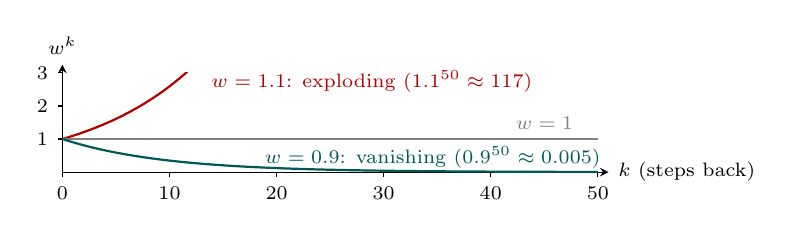
\begin{tikzpicture}[font=\scriptsize]
  \def\xs{0.136} \def\ys{0.42}
  \draw[->, >=stealth] (0, 0) -- ({51 * \xs}, 0) node[right] {$k$ (steps back)};
  \draw[->, >=stealth] (0, 0) -- (0, {3.25 * \ys}) node[above] {$w^k$};
  \foreach \v in {0, 10, 20, 30, 40, 50}{
    \draw ({\v * \xs}, 0) -- ({\v * \xs}, -0.06) node[below] {\v};
  }
  \foreach \v in {1, 2, 3}{
    \draw (0, {\v * \ys}) -- (-0.06, {\v * \ys}) node[left] {\v};
  }
  \begin{scope}
    \clip (0, 0) rectangle ({50 * \xs}, {3 * \ys});
    \draw[red!70!black, thick, domain=0:50, samples=80] plot ({\x * \xs}, {\ys * 1.1^\x});
    \draw[gray, thick] (0, \ys) -- ({50 * \xs}, \ys);
    \draw[teal!70!black, thick, domain=0:50, samples=80] plot ({\x * \xs}, {\ys * 0.9^\x});
  \end{scope}
  \node[anchor=west, red!70!black] at ({13 * \xs}, {2.75 * \ys}) {$w = 1.1$: exploding ($1.1^{50} \approx 117$)};
  \node[anchor=south, gray] at ({45 * \xs}, \ys) {$w = 1$};
  \node[anchor=west, teal!70!black] at ({18 * \xs}, {0.45 * \ys}) {$w = 0.9$: vanishing ($0.9^{50} \approx 0.005$)};
\end{tikzpicture}
\end{center}

\vfill

\end{frame}

% ------------------------------------------------------------------------------


\begin{frame}
\vfill
\medskip
\medskip
\centering\LARGE\bfseries What if the recurrence itself were linear?
\vfill
\end{frame}



% ------------------------------------------------------------------------------

\begin{frame}{Linear RNNs}

\vfill

\begin{itemize}
  \item Remove the non-linearity from the recurrence:
        \[ \vec h_t = \vec A \vec h_{t-1} + \vec B \vec x_t, \qquad \vec y_t = \vec C \vec h_t \]
  \item Non-linearities move \textbf{between} recurrent layers and act per position
  \item Same division of labor as in the transformer: one sub-layer mixes positions, one transforms each position
\end{itemize}

\vfill

\begin{center}
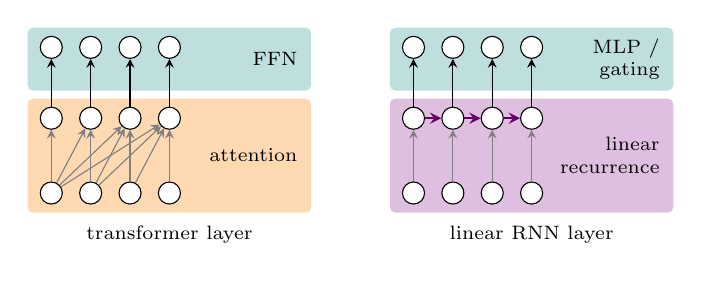
\begin{tikzpicture}[
    font=\scriptsize,
    nd/.style={circle, draw, fill=white, inner sep=0pt, minimum size=2.8mm},
    flow/.style={->, >=stealth},
  ]
  \foreach \ox/\mixname/\mixcol/\chname/\title/\kind in {
      0/{attention}/orange!30/{FFN}/{transformer layer}/attn,
      4.6/{linear\\recurrence}/violet!25/{MLP /\\gating}/{linear RNN layer}/rec}{
    % bands
    \fill[\mixcol, rounded corners=2pt] (\ox, -0.25) rectangle ++(3.6, 1.45);
    \fill[teal!25, rounded corners=2pt] (\ox, 1.3) rectangle ++(3.6, 0.8);
    \node[anchor=east, align=right] at (\ox + 3.55, 0.48) {\mixname};
    \node[anchor=east, align=right] at (\ox + 3.55, 1.7) {\chname};
    % tokens
    \foreach \p in {1,...,4}{
      \node[nd] (a\kind\p) at ({\ox + 0.3 + (\p - 1) * 0.5}, 0) {};
      \node[nd] (b\kind\p) at ({\ox + 0.3 + (\p - 1) * 0.5}, 0.95) {};
      \node[nd] (c\kind\p) at ({\ox + 0.3 + (\p - 1) * 0.5}, 1.85) {};
      \draw[flow] (b\kind\p) -- (c\kind\p);
    }
    \node[anchor=north] at (\ox + 1.8, -0.3) {\title};
  }
  % attention: every position reads all earlier positions
  \foreach \p in {1,...,4}{
    \foreach \s in {1,...,\p}{
      \draw[flow, gray] (aattn\s) -- (battn\p);
    }
  }
  % recurrence: input enters the state, state is passed on
  \foreach \p in {1,...,4}{
    \draw[flow, gray] (arec\p) -- (brec\p);
  }
  \foreach \p [remember=\p as \pp (initially 1)] in {2,...,4}{
    \draw[flow, thick, violet!80!black] (brec\pp) -- (brec\p);
  }
\end{tikzpicture}
\end{center}

\vfill

\end{frame}

% ------------------------------------------------------------------------------

\begin{frame}{A Linear RNN Is a Convolution}

\vfill

\begin{itemize}
  \item Unroll from $\vec h_0 = \vec 0$ (so $\vec h_1 = \vec B \vec x_1$) and read out with $\vec C$:
        \begin{align*}
          \vec h_2 &= \vec A \vec h_1 + \vec B \vec x_2 = \vec A \vec B\, \vec x_1 + \vec B\, \vec x_2\\
          \vec h_3 &= \vec A \vec h_2 + \vec B \vec x_3 = \vec A^2 \vec B\, \vec x_1 + \vec A \vec B\, \vec x_2 + \vec B\, \vec x_3\\
          \vec y_3 &= \vec C \vec h_3 = \underbrace{\vec C \vec A^2 \vec B}_{\vec K_2}\, \vec x_1 + \underbrace{\vec C \vec A \vec B}_{\vec K_1}\, \vec x_2 + \underbrace{\vec C \vec B}_{\vec K_0}\, \vec x_3
        \end{align*}
   \item The \textbf{kernel} collects the weights $\vec K_k = \vec C \vec A^k \vec B$ of tokens $k$ steps back:
        $\vec K = (\vec K_0, \vec K_1, \vec K_2, \ldots) = (\vec C \vec B,\ \vec C \vec A \vec B,\ \vec C \vec A^2 \vec B,\ \ldots)$
  \item Output: $\vec y_t = \sum_{k=0}^{t-1} \vec K_k\, \vec x_{t-k}$, which represents a 1D \textbf{convolution} over the input sequence with $\vec K$
  \item If $\vec A$ shrinks vectors, older tokens fade
\end{itemize}


\begin{center}
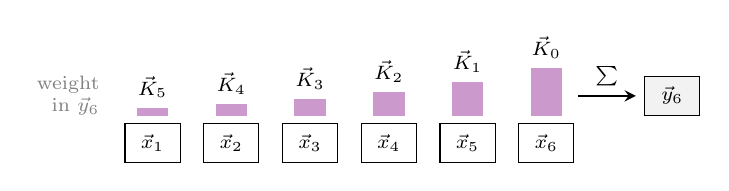
\begin{tikzpicture}[font=\scriptsize]
  \def\dx{1.0}
  \foreach \s in {1,...,6}{
    \pgfmathtruncatemacro{\k}{6 - \s}
    \pgfmathsetmacro{\hh}{0.6 * 0.7^\k}
    \node[draw, minimum width=7mm, minimum height=5mm, fill=white] (x\s) at ({\s * \dx}, 0) {$\vec x_{\s}$};
    \fill[violet!40] ({\s * \dx - 0.2}, 0.35) rectangle ++(0.4, \hh);
    \node[anchor=south] at ({\s * \dx}, {0.35 + \hh}) {$\vec K_{\k}$};
  }
  \node[draw, fill=gray!10, minimum width=7mm, minimum height=5mm] (y) at ({7.6 * \dx}, 0.6) {$\vec y_6$};
  \draw[->, >=stealth, thick] ({6.4 * \dx}, 0.6) -- node[above] {$\sum$} ([xshift=-3pt]y.west);
  \node[anchor=east, gray, align=right] at ({0.45 * \dx}, 0.6) {weight\\ in $\vec y_6$};
\end{tikzpicture}
\end{center}

\vfill

\end{frame}

% ------------------------------------------------------------------------------


\begin{frame}{Example: Sliding the Kernel}

\vfill

\begin{itemize}
  \item Scalar example: $A = 0.5$, $B = C = 1$ $\rightarrow$ kernel $K = (1,\ 0.5,\ 0.25,\ 0.125,\ \ldots)$
  \item Slide the kernel along the input: $K_0$ on the current token, $K_1$ on the one before, etc.
  \item Same result as running the recurrence $h_t = 0.5\, h_{t-1} + x_t$: \; $4,\ 4,\ 2,\ 3$
\end{itemize}

\medskip

\begin{center}
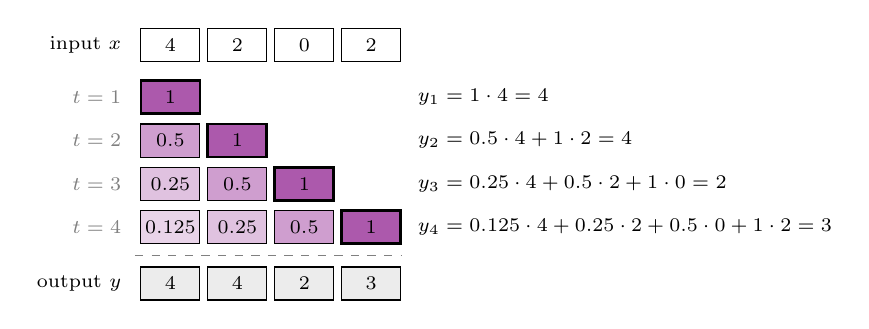
\begin{tikzpicture}[
    font=\scriptsize,
    cell/.style={draw, minimum width=7.5mm, minimum height=4.2mm, inner sep=0pt},
  ]
  \def\dx{0.85} \def\dy{0.55}
  % ---- input -------------------------------------------------------------------------------
  \node[anchor=east] at (0.35, 0) {input $x$};
  \foreach \v [count=\c] in {4, 2, 0, 2}{
    \node[cell, fill=white] at ({\c * \dx}, 0) {\v};
  }
  % ---- kernel positions for t = 1, ..., 4 --------------------------------------------------
  \foreach \t/\eq in {1/{$y_1 = 1 \cdot 4 = 4$},
                      2/{$y_2 = 0.5 \cdot 4 + 1 \cdot 2 = 4$},
                      3/{$y_3 = 0.25 \cdot 4 + 0.5 \cdot 2 + 1 \cdot 0 = 2$},
                      4/{$y_4 = 0.125 \cdot 4 + 0.25 \cdot 2 + 0.5 \cdot 0 + 1 \cdot 2 = 3$}}{
    \pgfmathsetmacro{\y}{-(\t + 0.2) * \dy}
    \node[anchor=east, gray] at (0.35, \y) {$t = \t$};
    \foreach \c in {1,...,\t}{
      \pgfmathtruncatemacro{\k}{\t - \c}
      \pgfmathsetmacro{\kv}{0.5^\k}
      \pgfmathtruncatemacro{\pc}{round(55 * 0.5^\k) + 10}
      \ifnum\k=0
        \node[cell, fill=violet!\pc, line width=1pt] at ({\c * \dx}, \y) {\pgfmathprintnumber[precision=3]{\kv}};
      \else
        \node[cell, fill=violet!\pc] at ({\c * \dx}, \y) {\pgfmathprintnumber[precision=3]{\kv}};
      \fi
    }
    \node[anchor=west] at ({4.55 * \dx}, \y) {\eq};
  }
  % ---- output ------------------------------------------------------------------------------
  \pgfmathsetmacro{\yo}{-5.5 * \dy}
  \node[anchor=east] at (0.35, \yo) {output $y$};
  \foreach \v [count=\c] in {4, 4, 2, 3}{
    \node[cell, fill=gray!15] at ({\c * \dx}, \yo) {\v};
  }
  \draw[gray, dashed] (0.4, {-4.85 * \dy}) -- ({4.45 * \dx}, {-4.85 * \dy});
\end{tikzpicture}
\end{center}

\vfill

\end{frame}



\begin{frame}{Parallel Training via Convolution}

\vfill

\begin{itemize}
  \item Training: compute $\vec K$ from the current $\vec A, \vec B, \vec C$ (once per step, shared by all sequences), then all outputs at once
  \item As a matrix: lower-triangular and constant along each diagonal
  \item Inference: run the recurrence, $O(1)$ per new token with a fixed-size state
  \item Requires same $\vec A, \vec B, \vec C$ at every step: \textbf{linear time-invariant} (LTI)
\end{itemize}

\vfill

\begin{center}
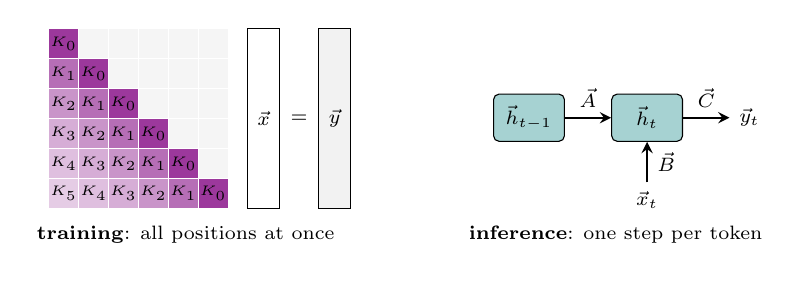
\begin{tikzpicture}[
    font=\scriptsize,
    vecbox/.style={draw, fill=white, minimum width=4mm, inner sep=0pt},
    flow/.style={->, >=stealth, thick},
  ]
  \def\cs{0.38}
  % ---- training: y = K x with a lower-triangular Toeplitz matrix ---------------------------
  \foreach \qq in {1,...,6}{
    \foreach \kk in {1,...,6}{
      \pgfmathsetmacro{\xx}{(\kk - 1) * \cs}
      \pgfmathsetmacro{\yy}{(6 - \qq) * \cs}
      \ifnum\kk>\qq
        \filldraw[fill=gray!8, draw=white, line width=0.4pt] (\xx, \yy) rectangle ++(\cs, \cs);
      \else
        \pgfmathtruncatemacro{\lag}{\qq - \kk}
        \pgfmathtruncatemacro{\pc}{round(70 * 0.7^\lag) + 8}
        \filldraw[fill=violet!\pc, draw=white, line width=0.4pt] (\xx, \yy) rectangle ++(\cs, \cs);
        \node[font=\tiny] at (\xx + \cs / 2, \yy + \cs / 2) {$K_{\lag}$};
      \fi
    }
  }
  \node[vecbox, minimum height={6 * \cs cm}] (xv) at ({6 * \cs + 0.45}, {3 * \cs}) {};
  \node at (xv) {$\vec x$};
  \node at ({6 * \cs + 0.9}, {3 * \cs}) {$=$};
  \node[vecbox, minimum height={6 * \cs cm}, fill=gray!10] (yv) at ({6 * \cs + 1.35}, {3 * \cs}) {};
  \node at (yv) {$\vec y$};
  \node[anchor=north, align=center] at ({3 * \cs + 0.6}, -0.1) {\textbf{training}: all positions at once};
  % ---- inference: recurrence -----------------------------------------------------------
  \begin{scope}[xshift=5.6cm]
    \node[draw, rounded corners=2pt, fill=teal!35, minimum width=9mm, minimum height=6mm] (hp) at (0.5, 1.15) {$\vec h_{t-1}$};
    \node[draw, rounded corners=2pt, fill=teal!35, minimum width=9mm, minimum height=6mm] (hc) at (2.0, 1.15) {$\vec h_t$};
    \node (xt) at (2.0, 0.1) {$\vec x_t$};
    \node (yt) at (3.3, 1.15) {$\vec y_t$};
    \draw[flow] (hp) -- node[above] {$\vec A$} (hc);
    \draw[flow] (xt) -- node[right] {$\vec B$} (hc);
    \draw[flow] (hc) -- node[above] {$\vec C$} (yt);
    \node[anchor=north, align=center] at (1.6, -0.1) {\textbf{inference}: one step per token};
  \end{scope}
\end{tikzpicture}
\end{center}

\vfill

\end{frame}





\begin{frame}{Two Ways to Parallelize}

\vfill

\begin{itemize}
  \item Computing $\vec K$ naively needs $n$ powers of the $N \times N$ matrix $\vec A$, which is very costly
  \item Option 1: FFT-based algorithms (works for LTI only)
  \item Option 2: compute all states directly with a \textbf{parallel scan}, which also works if $\vec A$ and $\vec B$ change per position (stay tuned!)
\end{itemize}

\vfill

\end{frame}

% ------------------------------------------------------------------------------

\begin{frame}{Parallel Scan Basics}

\vfill

\begin{itemize}
  \item A \textbf{scan} computes all running results of an operation
  \item Example for sum: $(3, 1, 4, 1, 5, 9, 2, 6) \rightarrow (3, 4, 8, 9, 14, 23, 25, 31)$ 
  \item Sequential scan: $n$ steps
  \item Parallel scan: each position adds the value $1, 2, 4, \ldots$ positions to its left $\rightarrow$ $\log_2 n$ steps
  \item Works for any \textbf{associative} operation, $(a \bullet b) \bullet c = a \bullet (b \bullet c)$
\end{itemize}

\medskip
\medskip

\begin{center}
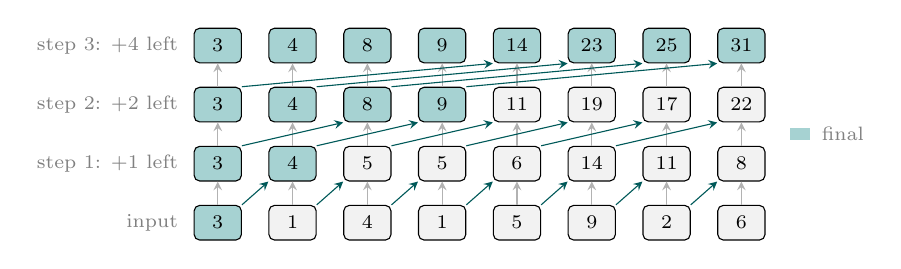
\begin{tikzpicture}[
    font=\scriptsize,
    el/.style={draw, rounded corners=2pt, inner sep=0pt, minimum width=6mm, minimum height=4.4mm},
    done/.style={el, fill=teal!35},
    open/.style={el, fill=gray!10},
    flow/.style={->, >=stealth, teal!70!black},
  ]
  \def\dx{0.95} \def\dy{0.75}
  % running sums of 3 1 4 1 5 9 2 6; teal = final value
  \foreach \lay/\vals in {0/{3,1,4,1,5,9,2,6}, 1/{3,4,5,5,6,14,11,8},
                          2/{3,4,8,9,11,19,17,22}, 3/{3,4,8,9,14,23,25,31}}{
    \foreach \v [count=\p] in \vals {
      \pgfmathtruncatemacro{\done}{\p <= 2^\lay}
      \ifnum\done=1
        \node[done] (n\lay-\p) at ({\p * \dx}, {\lay * \dy}) {\v};
      \else
        \node[open] (n\lay-\p) at ({\p * \dx}, {\lay * \dy}) {\v};
      \fi
    }
  }
  \foreach \lay/\dist in {1/1, 2/2, 3/4}{
    \pgfmathtruncatemacro{\pl}{\lay - 1}
    \foreach \p in {1,...,8}{
      \draw[->, >=stealth, gray!60] (n\pl-\p) -- (n\lay-\p);
      \pgfmathtruncatemacro{\src}{\p - \dist}
      \ifnum\src>0
        \draw[flow] (n\pl-\src.north east) -- (n\lay-\p.south west);
      \fi
    }
  }
  \foreach \lay/\lab in {0/input, 1/{step 1: $+1$ left}, 2/{step 2: $+2$ left}, 3/{step 3: $+4$ left}}{
    \node[anchor=east, gray] at ({0.6 * \dx}, {\lay * \dy}) {\lab};
  }
  \fill[teal!35] ({8.65 * \dx}, {1.5 * \dy - 0.08}) rectangle ++(0.25, 0.16);
  \node[anchor=west, gray] at ({8.65 * \dx + 0.28}, {1.5 * \dy}) {final};
\end{tikzpicture}
\end{center}

\vfill

\end{frame}

% ------------------------------------------------------------------------------

\begin{frame}{Parallel Scan for Linear RNNs}

\vfill

\begin{itemize}

  \item One step: multiply the state by $\vec A$, then add $\vec b_t = \vec B \vec x_t$
  \item Two steps have the same form:
        \[ \vec A_2 (\vec A_1 \vec h + \vec b_1) + \vec b_2 = \vec A_2 \vec A_1\, \vec h + (\vec A_2 \vec b_1 + \vec b_2) \]
  \item A pair $(\vec A, \vec b)$ summarizes a block of steps, with pairs combining like numbers in a sum: $(\vec A_1, \vec b_1) \bullet (\vec A_2, \vec b_2) = (\vec A_2 \vec A_1,\ \vec A_2 \vec b_1 + \vec b_2)$ 
  \item Problem: each combination is a costly $N \times N$ matrix product
\end{itemize}

\medskip

\begin{center}
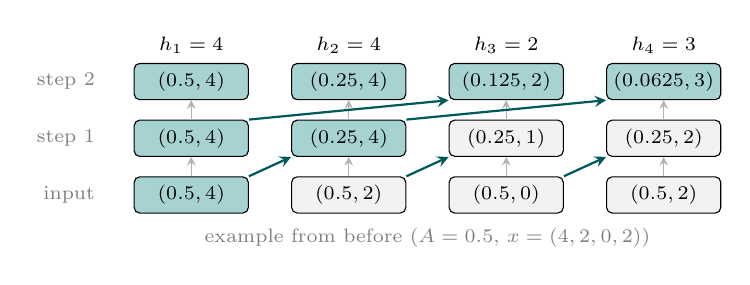
\begin{tikzpicture}[
    font=\scriptsize,
    el/.style={draw, rounded corners=2pt, inner sep=2pt, minimum width=1.45cm, minimum height=4.6mm},
    done/.style={el, fill=teal!35},
    open/.style={el, fill=gray!10},
    flow/.style={->, >=stealth, teal!70!black, thick},
  ]
  \def\dx{2.0} \def\dy{0.72}
  % rows: input, step 1, step 2; teal = state is final
  \foreach \lay/\vals in {0/{(0.5, 4)/1, (0.5, 2)/0, (0.5, 0)/0, (0.5, 2)/0},
                          1/{(0.5, 4)/1, (0.25, 4)/1, (0.25, 1)/0, (0.25, 2)/0},
                          2/{(0.5, 4)/1, (0.25, 4)/1, (0.125, 2)/1, (0.0625, 3)/1}}{
    \foreach \v/\d [count=\p] in \vals {
      \ifnum\d=1
        \node[done] (n\lay-\p) at ({\p * \dx}, {\lay * \dy}) {$\v$};
      \else
        \node[open] (n\lay-\p) at ({\p * \dx}, {\lay * \dy}) {$\v$};
      \fi
    }
  }
  % step 1: combine with the neighbor 1 to the left; step 2: 2 to the left
  \foreach \lay/\dist in {1/1, 2/2}{
    \pgfmathtruncatemacro{\pl}{\lay - 1}
    \foreach \p in {1,...,4}{
      \draw[->, >=stealth, gray!60] (n\pl-\p) -- (n\lay-\p);
      \pgfmathtruncatemacro{\src}{\p - \dist}
      \ifnum\src>0
        \draw[flow] (n\pl-\src.north east) -- (n\lay-\p.south west);
      \fi
    }
  }
  \foreach \lay/\lab in {0/input, 1/step 1, 2/step 2}{
    \node[anchor=east, gray] at ({0.45 * \dx}, {\lay * \dy}) {\lab};
  }
  \foreach \h [count=\p] in {4, 4, 2, 3}{
    \node[anchor=south] at (n2-\p.north) {$h_{\p} = \h$};
  }
  \node[anchor=north, gray, align=center] at ({2.5 * \dx}, -0.3) {example from before ($A = 0.5$, $x = (4, 2, 0, 2)$)};
\end{tikzpicture}
\end{center}

\vfill

\end{frame}


\begin{frame}{Why the Parallel Scan Is Faster}

\vfill

\begin{itemize}
  \item Sequential: every addition waits for the previous one $\rightarrow$ $n$ steps, one unit busy at a time
  \item Parallel scan: more additions in total, but only $\log_2 n$ dependent steps (e.g., with $n = 1024$: 10 instead of 1024)
  \item GPUs have thousands of units: idle units are free, waiting is not
\end{itemize}

\medskip
\medskip


\begin{center}
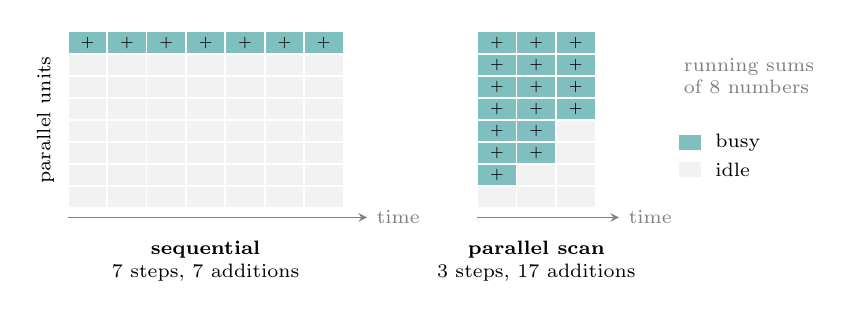
\begin{tikzpicture}[font=\scriptsize]
  \def\cw{0.5} \def\ch{0.28}
  % running sums of 8 numbers; teal = unit busy with an addition (busy units listed from the top)
  \foreach \ox/\ncols/\kind in {0/7/0, 5.2/3/1}{
    \foreach \st in {1,...,\ncols}{
      \foreach \u in {1,...,8}{
        \ifnum\kind=0
          \pgfmathtruncatemacro{\busy}{\u == 1}
        \else
          \pgfmathtruncatemacro{\busy}{(\st == 1 && \u <= 7) || (\st == 2 && \u <= 6) || (\st == 3 && \u <= 4)}
        \fi
        \ifnum\busy=1
          \filldraw[fill=teal!50, draw=white, line width=0.6pt] ({\ox + (\st - 1) * \cw}, {(8 - \u) * \ch}) rectangle ++(\cw, \ch);
          \node[font=\tiny] at ({\ox + (\st - 0.5) * \cw}, {(8.5 - \u) * \ch}) {$+$};
        \else
          \filldraw[fill=gray!10, draw=white, line width=0.6pt] ({\ox + (\st - 1) * \cw}, {(8 - \u) * \ch}) rectangle ++(\cw, \ch);
        \fi
      }
    }
    \draw[->, >=stealth, gray] (\ox, -0.12) -- ({\ox + \ncols * \cw + 0.3}, -0.12) node[right] {time};
  }
  \node[anchor=south, rotate=90] at (-0.05, {4 * \ch}) {parallel units};
  \node[anchor=north, align=center] at ({3.5 * \cw}, -0.3) {\textbf{sequential}\\ 7 steps, 7 additions};
  \node[anchor=north, align=center] at ({5.2 + 1.5 * \cw}, -0.3) {\textbf{parallel scan}\\ 3 steps, 17 additions};
  \node[anchor=west, gray, align=left] at ({5.2 + 3 * \cw + 1.0}, {6 * \ch}) {running sums\\ of 8 numbers};
  \filldraw[fill=teal!50, draw=white] ({5.2 + 3 * \cw + 1.05}, {2.6 * \ch}) rectangle ++(0.3, 0.2);
  \node[anchor=west] at ({5.2 + 3 * \cw + 1.4}, {2.6 * \ch + 0.1}) {busy};
  \filldraw[fill=gray!10, draw=white] ({5.2 + 3 * \cw + 1.05}, {1.4 * \ch}) rectangle ++(0.3, 0.2);
  \node[anchor=west] at ({5.2 + 3 * \cw + 1.4}, {1.4 * \ch + 0.1}) {idle};
\end{tikzpicture}
\end{center}

\vfill

\end{frame}


\begin{frame}{Diagonalization}

\vfill

\begin{itemize}
  \item Most matrices can be written as $\vec A = \vec P \vec \Lambda \vec P^{-1}$, with the eigenvalues on the diagonal of $\vec \Lambda = \mathrm{diag}(\lambda_1, \ldots, \lambda_N)$, e.g.
        \[ \underbrace{\begin{pmatrix} 0.6 & 0.2 \\ 0.2 & 0.6 \end{pmatrix}}_{\vec A}
           = \underbrace{\begin{pmatrix} 1 & 1 \\ 1 & -1 \end{pmatrix}}_{\vec P}
             \underbrace{\begin{pmatrix} \org{0.8} & 0 \\ 0 & \org{0.4} \end{pmatrix}}_{\vec \Lambda}
             \underbrace{\begin{pmatrix} 0.5 & 0.5 \\ 0.5 & -0.5 \end{pmatrix}}_{\vec P^{-1}} \]
  \item In products, the inner $\vec P^{-1} \vec P$ cancel:
        \[ \vec A^2 = \vec P \vec \Lambda \underbrace{\vec P^{-1} \vec P}_{\vec I} \vec \Lambda \vec P^{-1} = \vec P \vec \Lambda^2 \vec P^{-1},
           \qquad \vec A^k = \vec P \vec \Lambda^k \vec P^{-1} \]
  \item Only the diagonal is raised to the power: $\vec \Lambda^k = \mathrm{diag}(\lambda_1^k, \ldots, \lambda_N^k)$
\end{itemize}

\vfill

\end{frame}


\begin{frame}{Diagonal Linear RNNs}

\vfill

\begin{itemize}
  \item Diagonalize $\vec A = \vec P \vec \Lambda \vec P^{-1}$ and absorb $\vec P^{-1}$ into $\vec B$ and $\vec P$ into $\vec C$: we simply learn the diagonal $\vec \lambda = (\lambda_1, \ldots, \lambda_N)$
  \item The recurrence becomes element-wise:
        \[ \vec h_t = \vec \lambda \odot \vec h_{t-1} + \vec B \vec x_t \]
  \item So does the scan operator, with $N$ instead of $N^3$ operations per combination:
        \[ (\vec a_1, \vec b_1) \bullet (\vec a_2, \vec b_2) = (\vec a_2 \odot \vec a_1,\ \vec a_2 \odot \vec b_1 + \vec b_2) \]
\end{itemize}

\vfill

\begin{center}
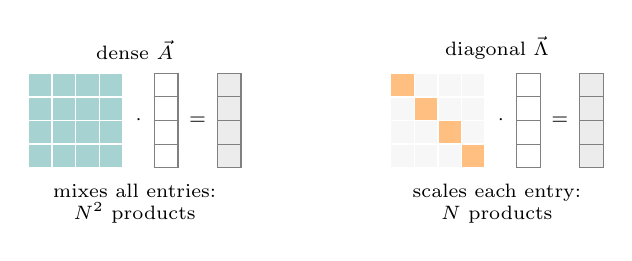
\begin{tikzpicture}[font=\scriptsize]
  \def\cs{0.3}
  \foreach \ox/\isdiag/\title/\note in {0/0/{dense $\vec A$}/{mixes all entries:\\ $N^2$ products},
                                        4.6/1/{diagonal $\vec \Lambda$}/{scales each entry:\\ $N$ products}}{
    % matrix
    \foreach \r in {1,...,4}{
      \foreach \c in {1,...,4}{
        \ifnum\isdiag=1
          \ifnum\r=\c \def\mcol{orange!50} \else \def\mcol{gray!6} \fi
        \else
          \def\mcol{teal!35}
        \fi
        \filldraw[fill=\mcol, draw=white, line width=0.5pt] ({\ox + (\c - 1) * \cs}, {(4 - \r) * \cs}) rectangle ++(\cs, \cs);
      }
    }
    % times h = result
    \node at ({\ox + 4 * \cs + 0.2}, {2 * \cs}) {$\cdot$};
    \foreach \r in {1,...,4}{
      \filldraw[fill=white, draw=gray] ({\ox + 4 * \cs + 0.4}, {(4 - \r) * \cs}) rectangle ++(\cs, \cs);
      \filldraw[fill=gray!15, draw=gray] ({\ox + 5 * \cs + 0.9}, {(4 - \r) * \cs}) rectangle ++(\cs, \cs);
    }
    \node at ({\ox + 5 * \cs + 0.65}, {2 * \cs}) {$=$};
    \node[anchor=south] at ({\ox + 3 * \cs + 0.45}, {4 * \cs + 0.05}) {\title};
    \node[anchor=north, align=center] at ({\ox + 3 * \cs + 0.45}, -0.08) {\note};
  }
\end{tikzpicture}
\end{center}

\vfill

\end{frame}

% ------------------------------------------------------------------------------





\begin{frame}{Gradients in Linear RNNs}

\vfill

\begin{itemize}
  \item Since $\vec h_t = \vec \lambda \odot \vec h_{t-1} + \vec B \vec x_t$, each chain rule step contributes just $\vec \lambda$:
        \[ \frac{\partial \vec h_3}{\partial \vec h_0}
           = \underbrace{\frac{\partial \vec h_3}{\partial \vec h_2}}_{\vec \lambda}\,
             \underbrace{\frac{\partial \vec h_2}{\partial \vec h_1}}_{\vec \lambda}\,
             \underbrace{\frac{\partial \vec h_1}{\partial \vec h_0}}_{\vec \lambda}
           = \vec \lambda^3 \quad \text{(element-wise)} \]
  \item $|\lambda_i| < 1$: no explosion, near 1: long memory $\rightarrow$ choose $\lambda_i$ carefully
\end{itemize}

\medskip
\medskip

\begin{center}
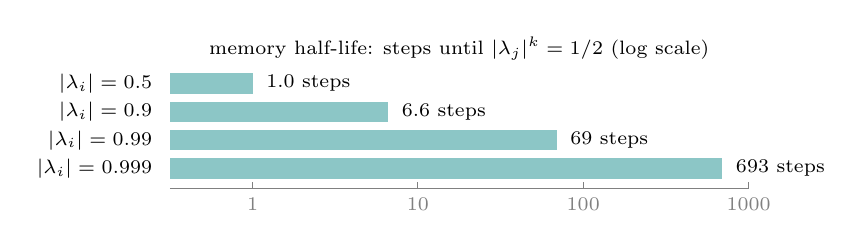
\begin{tikzpicture}[font=\scriptsize]
  \def\sc{2.1}  % cm per decade; axis from 10^-0.5 to 10^3
  % half-life = ln 2 / -ln |lambda|
  \foreach \lam/\hl [count=\r] in {0.5/1.0, 0.9/6.6, 0.99/69, 0.999/693}{
    \pgfmathsetmacro{\y}{-(\r - 1) * 0.36}
    \pgfmathsetmacro{\xx}{\sc * (log10(\hl) + 0.5)}
    \fill[teal!45] (0, \y) rectangle (\xx, \y + 0.26);
    \node[anchor=east] at (-0.1, \y + 0.13) {$|\lambda_i| = \lam$};
    \node[anchor=west] at (\xx + 0.05, \y + 0.13) {\hl\ steps};
  }
  \draw[gray] (0, -1.2) -- ({\sc * 3.5}, -1.2);
  \foreach \v in {1, 10, 100, 1000}{
    \pgfmathsetmacro{\xx}{\sc * (log10(\v) + 0.5)}
    \draw[gray] (\xx, -1.2) -- (\xx, -1.12);
    \node[anchor=north, gray] at (\xx, -1.2) {\v};
  }
  \node[anchor=south] at ({\sc * 1.75}, 0.3) {memory half-life: steps until $|\lambda_j|^k = 1/2$ (log scale)};
\end{tikzpicture}
\end{center}

\vfill

\end{frame}

% ------------------------------------------------------------------------------

\begin{frame}{The Linear Recurrent Unit (LRU)}

\vfill

\begin{itemize}
  \item \textbf{Stable parameterization}: learn $\nu_i$ freely and set $\lambda_i = \exp(-\exp(\nu_i)) \in (0, 1)$ \citebutton{Orvieto et al. (2023) \cite{orvieto2023resurrecting}}{https://arxiv.org/abs/2303.06349}
  \item \textbf{Initialization} close to 1 (e.g., $0.9 \le \lambda_i \le 0.999$): long memory from the start
  \item \textbf{Normalization}: scale the input by $\gamma_i = \sqrt{1 - \lambda_i^2}$, so the state stays bounded as $\lambda_i \to 1$
  \item The LRU uses complex $\lambda_i$ (adds oscillations)
\end{itemize}

\vfill

\begin{center}
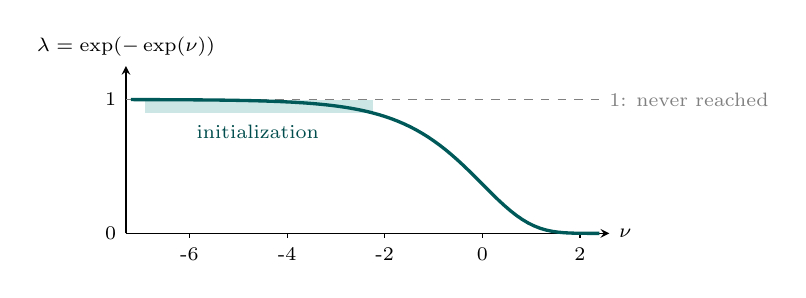
\begin{tikzpicture}[font=\scriptsize]
  \def\xs{0.62} \def\ys{1.7}
  % init band 0.9 <= lambda <= 0.999, i.e., -6.9 <= nu <= -2.25
  \fill[teal!20] ({-6.9 * \xs}, {0.9 * \ys}) rectangle ({-2.25 * \xs}, {0.999 * \ys});
  \draw[->, >=stealth] ({-7.3 * \xs}, 0) -- ({2.6 * \xs}, 0) node[right] {$\nu$};
  \draw[->, >=stealth] ({-7.3 * \xs}, 0) -- ({-7.3 * \xs}, {1.25 * \ys}) node[above] {$\lambda = \exp(-\exp(\nu))$};
  \draw[gray, dashed] ({-7.3 * \xs}, \ys) -- ({2.4 * \xs}, \ys) node[right] {1: never reached};
  \node[anchor=east] at ({-7.3 * \xs}, \ys) {1};
  \node[anchor=east] at ({-7.3 * \xs}, 0) {0};
  \foreach \v in {-6, -4, -2, 0, 2}{
    \draw ({\v * \xs}, 0) -- ({\v * \xs}, -0.06) node[below] {\v};
  }
  \draw[teal!70!black, very thick, domain=-7.2:2.4, samples=80] plot ({\x * \xs}, {\ys * exp(-exp(\x))});
  \node[anchor=north, teal!60!black] at ({-4.6 * \xs}, {0.88 * \ys}) {initialization};
\end{tikzpicture}
\end{center}

\vfill

\end{frame}

% ------------------------------------------------------------------------------


\begin{frame}{From a Vanilla RNN to the LRU}

\vfill

\begin{itemize}
  \item Step by step on Long Range Arena: tanh RNN $\rightarrow$ linear $\rightarrow$ complex diagonal $\rightarrow$ stable parameterization $\rightarrow$ normalization
  \item Long-range tasks such as PathX (16K tokens) need eigenvalues close to 1 and normalization
\end{itemize}


\medskip
\medskip


\centering
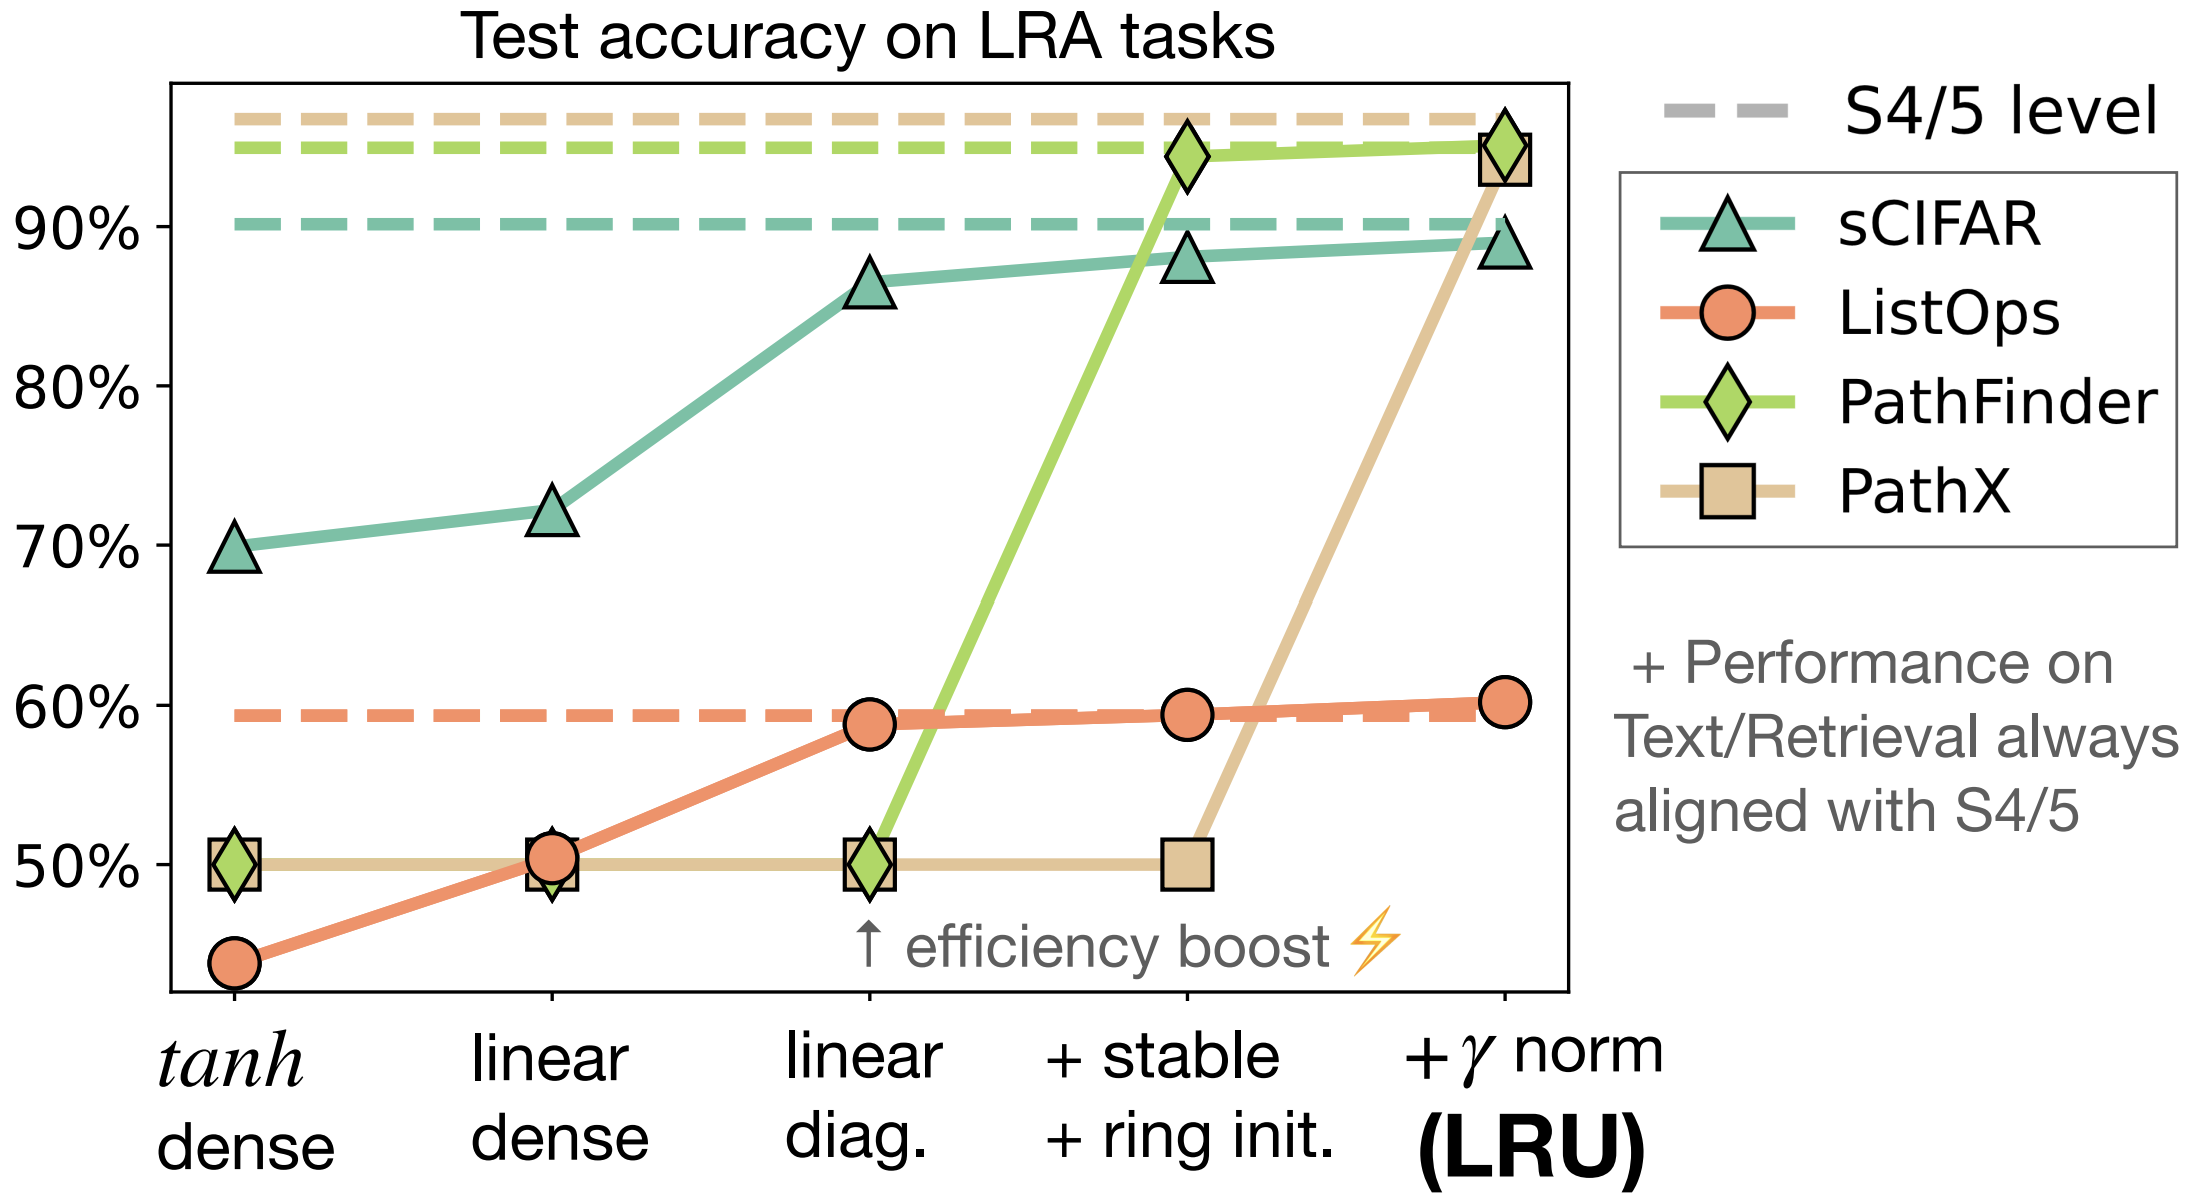
\includegraphics[width=0.7\textwidth]{figure/lru_steps.png}\\
\citebutton{Orvieto et al. (2023) \cite{orvieto2023resurrecting}}{https://arxiv.org/abs/2303.06349}

\vfill

\end{frame}



\begin{frame}{Example Task: PathFinder}

\vfill

\begin{itemize}
\item Are two points connected by a line or not
\item This is very far from language modeling!
\end{itemize}

\medskip
\medskip
\medskip

\centering
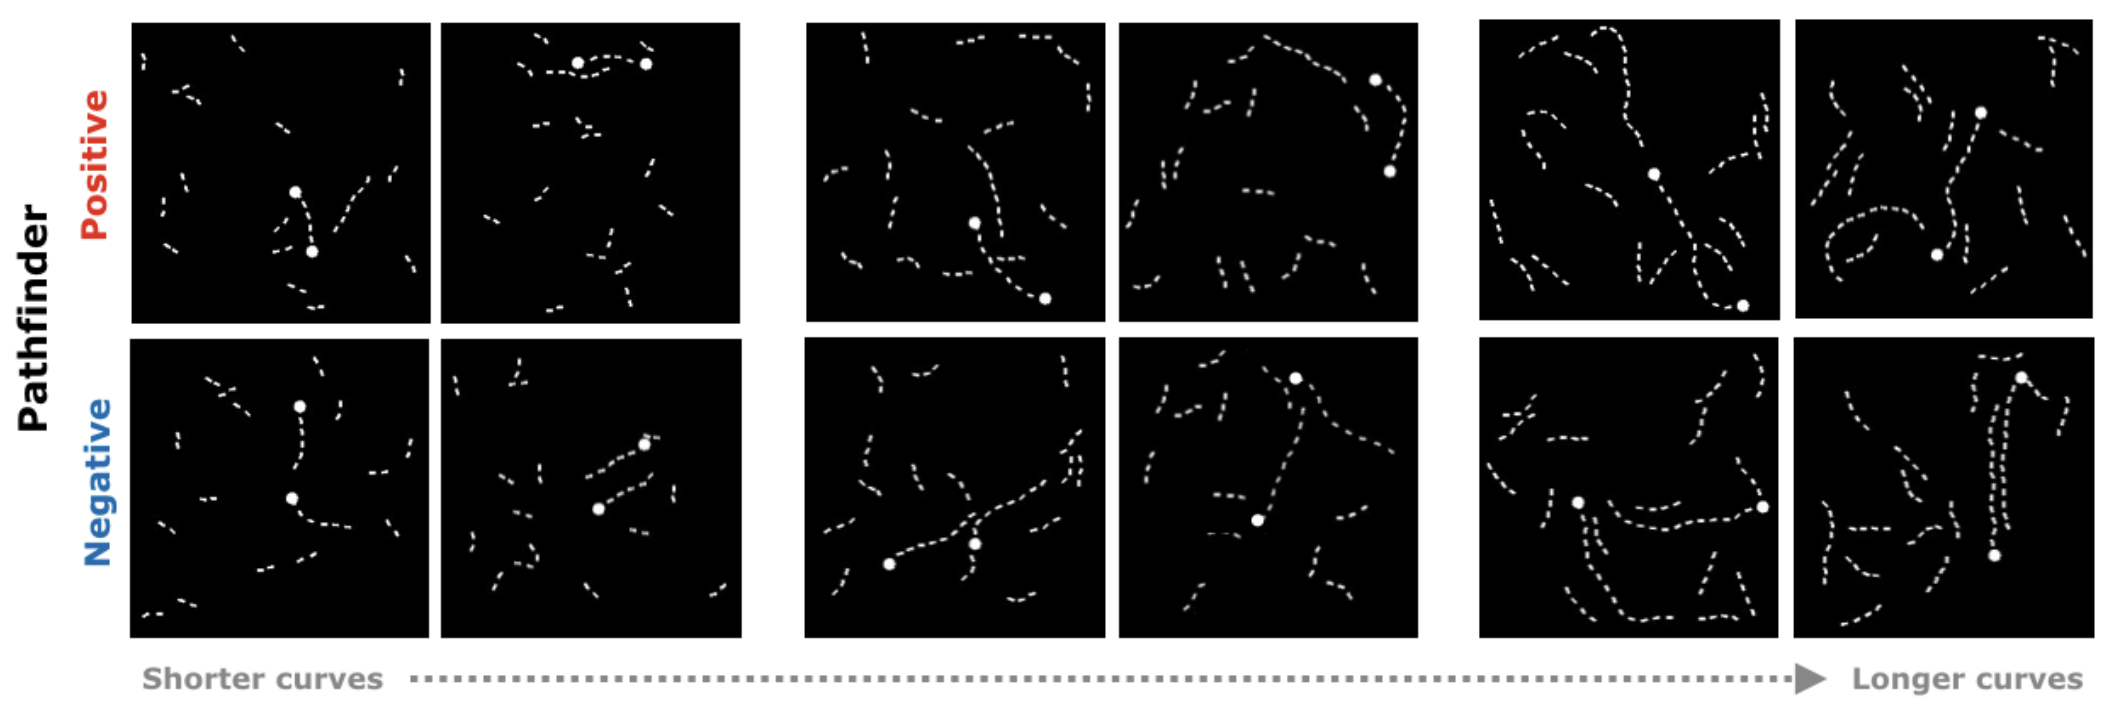
\includegraphics[width=0.9\textwidth]{figure/pathfinder.png}
\vfill

\end{frame}

% ------------------------------------------------------------------------------



\begin{frame}{Linear RNNs Are State Space Models}

\vfill

\begin{itemize}
  \item \textbf{State space models} (SSMs) from control theory: continuous-time linear dynamics
        \[ \vec h'(\tau) = \vec A \vec h(\tau) + \vec B x(\tau), \qquad y(\tau) = \vec C \vec h(\tau) \]
  \item Sampling with \textbf{step size} $\Delta$ gives a linear RNN:
        \begin{align*}
          \vec h_t &= \bar{\vec A} \vec h_{t-1} + \bar{\vec B} x_t\\
          \bar{\vec A} &= \exp(\Delta \vec A), \qquad
          \bar{\vec B} = (\Delta \vec A)^{-1}\big(\exp(\Delta \vec A) - \vec I\big)\, \Delta \vec B \approx \Delta \vec B
        \end{align*}
  \item SSM layers run one such system per channel $x$ of the input
\end{itemize}

\medskip
\medskip

\begin{center}
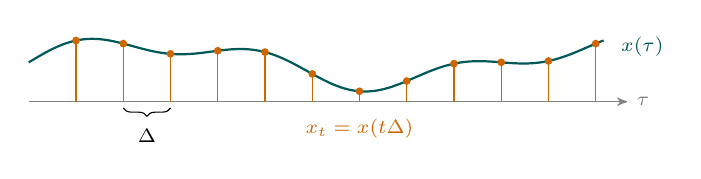
\begin{tikzpicture}[font=\scriptsize]
  \draw[->, gray] (0, 0) -- (7.6, 0) node[right] {$\tau$};
  \draw[thick, teal!70!black, domain=0:7.3, samples=120, smooth]
    plot (\x, {0.5 + 0.25 * sin(\x * 60) + 0.13 * sin(\x * 150)});
  \foreach \k in {1,...,12}{
    \pgfmathsetmacro{\xx}{\k * 0.6}
    \pgfmathsetmacro{\yy}{0.5 + 0.25 * sin(\xx * 60) + 0.13 * sin(\xx * 150)}
    \draw[orange!80!black] (\xx, 0) -- (\xx, \yy);
    \fill[orange!80!black] (\xx, \yy) circle (1.4pt);
  }
  \draw[decorate, decoration={brace, amplitude=3pt, mirror}] (1.2, -0.08) -- (1.8, -0.08) node[midway, below=4pt] {$\Delta$};
  \node[anchor=west, teal!70!black] at (7.4, 0.7) {$x(\tau)$};
  \node[anchor=north, orange!80!black] at (4.2, -0.1) {$x_t = x(t\Delta)$};
\end{tikzpicture}
\end{center}

\vfill

\end{frame}

% ------------------------------------------------------------------------------

\begin{frame}{Three Approaches to Linear Recurrence}

\vfill

\begin{itemize}
  \item S4 (Structured State Space Sequence Model): first model to solve PathX \citebutton{Gu et al. (2022) \cite{gu2022s4}}{https://arxiv.org/abs/2111.00396}
  \item Since then, many variants from three directions: SSMs, linear RNNs, linear attention (not covered)
  \item They differ in how $\vec A$ is structured and whether $\vec A, \vec B, \vec C$ depend on the input
\end{itemize}

\medskip
\medskip


\begin{center}
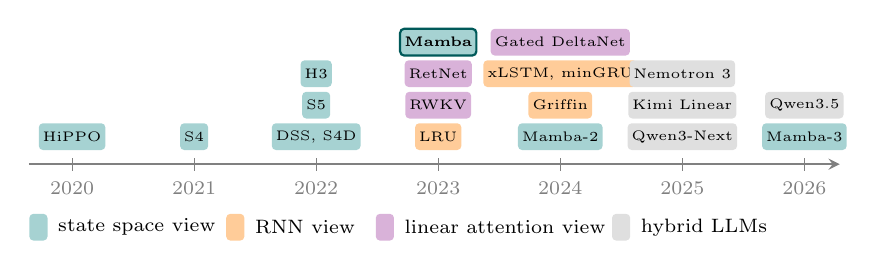
\begin{tikzpicture}[
    font=\scriptsize,
    m/.style={rounded corners=1.5pt, inner sep=1.5pt, minimum height=3.4mm, font=\tiny},
    ssm/.style={m, fill=teal!35},
    rnn/.style={m, fill=orange!40},
    lin/.style={m, fill=violet!30},
    hyb/.style={m, fill=gray!25},
  ]
  \draw[->, >=stealth, thick, gray] (0, 0) -- (10.3, 0);
  \foreach \yr [count=\i] in {2020,...,2026}{
    \pgfmathsetmacro{\x}{0.55 + (\i - 1) * 1.55}
    \draw[gray] (\x, -0.08) -- (\x, 0.08);
    \node[anchor=north, gray] at (\x, -0.1) {\yr};
  }
  % year positions: 2020 0.55, 2021 2.10, 2022 3.65, 2023 5.20, 2024 6.75, 2025 8.30, 2026 9.85
  \node[ssm] at (0.55, 0.35) {HiPPO};
  \node[ssm] at (2.10, 0.35) {S4};
  \node[ssm] at (3.65, 0.35) {DSS, S4D};
  \node[ssm] at (3.65, 0.75) {S5};
  \node[ssm] at (3.65, 1.15) {H3};
  \node[rnn] at (5.20, 0.35) {LRU};
  \node[lin] at (5.20, 0.75) {RWKV};
  \node[lin] at (5.20, 1.15) {RetNet};
  \node[ssm, draw=teal!70!black, thick] at (5.20, 1.55) {\textbf{Mamba}};
  \node[ssm] at (6.75, 0.35) {Mamba-2};
  \node[rnn] at (6.75, 0.75) {Griffin};
  \node[rnn] at (6.75, 1.15) {xLSTM, minGRU};
  \node[lin] at (6.75, 1.55) {Gated DeltaNet};
  \node[hyb] at (8.30, 0.35) {Qwen3-Next};
  \node[hyb] at (8.30, 0.75) {Kimi Linear};
  \node[hyb] at (8.30, 1.15) {Nemotron 3};
  \node[ssm] at (9.85, 0.35) {Mamba-3};
  \node[hyb] at (9.85, 0.75) {Qwen3.5};
  % legend
  \foreach \st/\lab/\x in {ssm/state space view/0, rnn/RNN view/2.5, lin/linear attention view/4.4, hyb/hybrid LLMs/7.4}{
    \node[\st, anchor=west] at (\x, -0.8) {\phantom{x}};
    \node[anchor=west] at (\x + 0.25, -0.8) {\lab};
  }
\end{tikzpicture}
\end{center}

\vfill

\end{frame}


\begin{frame}
\vfill
\medskip
\medskip
\centering\LARGE\bfseries Linear RNNs as discussed so far are relatively weak language models!
\vfill
\end{frame}



\section{Mamba}



\begin{frame}{What LTI Models Cannot Do}

\vfill

\begin{itemize}
  \item LTI: the same $\vec A, \vec B, \vec C$ are used for every token $\rightarrow$ the model cannot decide based on \textbf{content} what to store or skip
  \item \textbf{Selective copying}: reproduce the colored tokens, ignore the filler tokens in between
  \item A fixed kernel can only copy with fixed spacing
\end{itemize}

\medskip
\medskip
\medskip

\centering
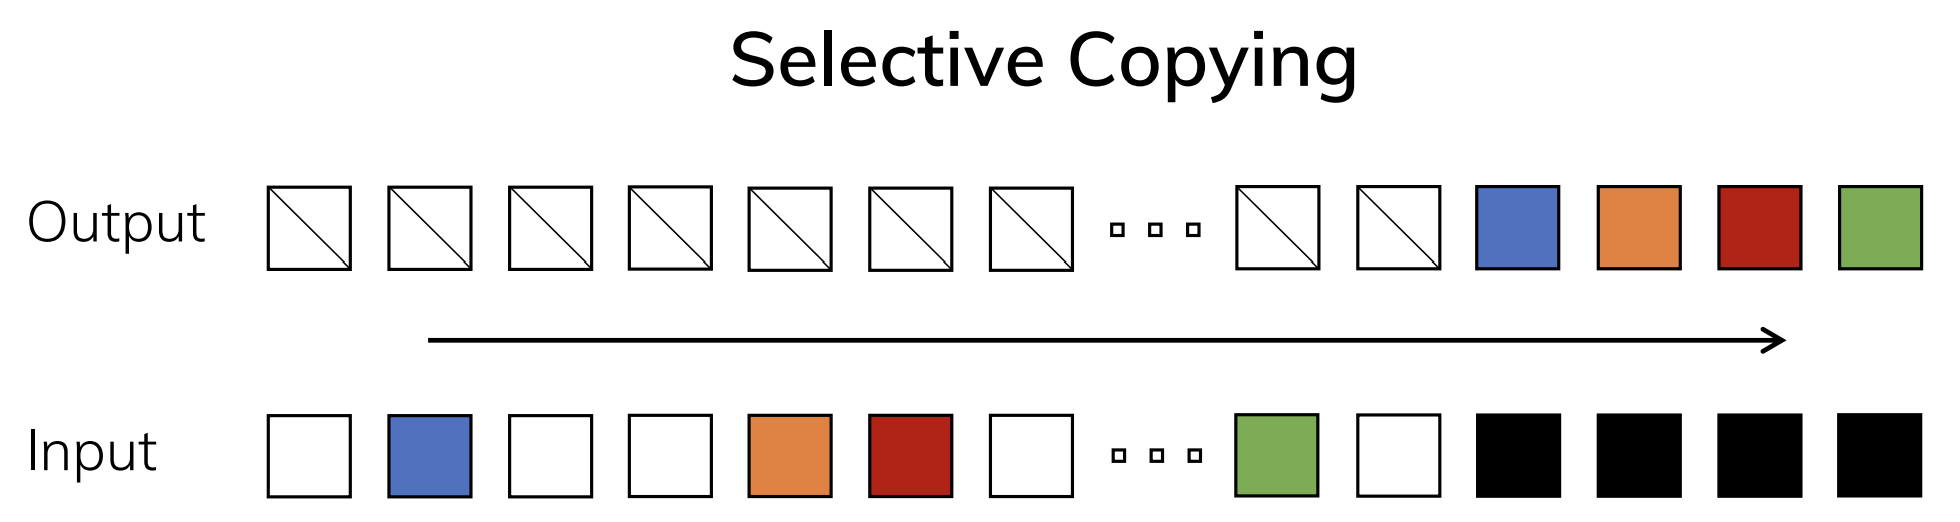
\includegraphics[width=0.9\textwidth]{figure/copying.png}

\vfill

\end{frame}

% ------------------------------------------------------------------------------

\begin{frame}{Selective State Space Models}

\vfill

\begin{itemize}
  \item \textbf{Selection}: $\vec B$, $\vec C$ and the step size $\Delta$ become functions of the current token \citebutton{Gu and Dao (2024) \cite{gu2024mamba}}{https://arxiv.org/abs/2312.00752}
        \[ \vec B_t = \vec W_B \vec x_t, \quad \vec C_t = \vec W_C \vec x_t, \quad \Delta_t = \mathrm{softplus}(\vec w_\Delta^\top \vec x_t + b_\Delta) \]
    \item For each channel $x_t$ of $\vec x_t$: \; $\vec h_t = \bar{\vec A}_t \vec h_{t-1} + \bar{\vec B}_t\, x_t, \quad y_t = \vec C_t^\top \vec h_t$, \; with $\bar{\vec A}_t, \bar{\vec B}_t$ discretized from $\vec A, \vec B_t$ using $\Delta_t$ (as before)
  \item Time-varying $\rightarrow$ no convolution kernel, but scan still works
\end{itemize}

\medskip
\medskip

\begin{center}
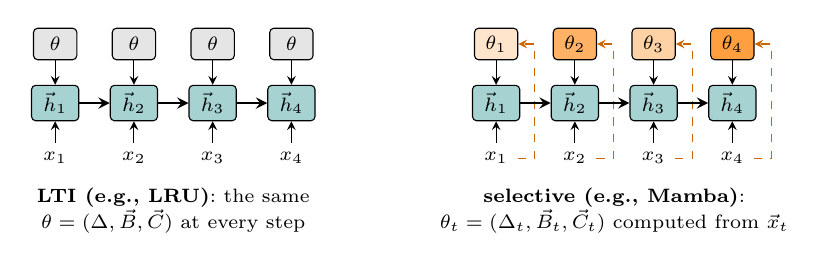
\begin{tikzpicture}[
    font=\scriptsize,
    st/.style={draw, rounded corners=1.5pt, fill=teal!35, minimum width=6mm, minimum height=4.5mm, inner sep=1pt},
    par/.style={draw, rounded corners=1.5pt, minimum width=5.5mm, minimum height=4mm, inner sep=1pt},
    flow/.style={->, >=stealth},
  ]
  % ---- LTI (S4) -------------------------------------------------------------------------
  \foreach \p in {1,...,4}{
    \node[st] (a\p) at ({(\p - 1) * 1.0}, 0) {$\vec h_{\p}$};
    \node (ax\p) at ({(\p - 1) * 1.0}, -0.7) {$x_{\p}$};
    \node[par, fill=gray!20] (ap\p) at ({(\p - 1) * 1.0}, 0.75) {$\theta$};
    \draw[flow] (ax\p) -- (a\p);
    \draw[flow] (ap\p) -- (a\p);
  }
  \foreach \p [remember=\p as \pp (initially 1)] in {2,...,4}{ \draw[flow, thick] (a\pp) -- (a\p); }
  \node[anchor=north, align=center] at (1.5, -0.95) {\textbf{LTI (e.g., LRU)}: the same\\ $\theta = (\Delta, \vec B, \vec C)$ at every step};
  % ---- selective (Mamba) -------------------------------------------------------------------
  \foreach \p/\pc in {1/20, 2/60, 3/35, 4/75}{
    \node[st] (b\p) at ({5.6 + (\p - 1) * 1.0}, 0) {$\vec h_{\p}$};
    \node (bx\p) at ({5.6 + (\p - 1) * 1.0}, -0.7) {$x_{\p}$};
    \node[par, fill=orange!\pc] (bp\p) at ({5.6 + (\p - 1) * 1.0}, 0.75) {$\theta_{\p}$};
    \draw[flow] (bx\p) -- (b\p);
    \draw[flow] (bp\p) -- (b\p);
    \draw[flow, dashed, orange!80!black] (bx\p.east) -- ++(0.22, 0) |- (bp\p.east);
  }
  \foreach \p [remember=\p as \pp (initially 1)] in {2,...,4}{ \draw[flow, thick] (b\pp) -- (b\p); }
  \node[anchor=north, align=center] at (7.1, -0.95) {\textbf{selective (e.g., Mamba)}:\\ $\theta_t = (\Delta_t, \vec B_t, \vec C_t)$ computed from $\vec x_t$};
\end{tikzpicture}
\end{center}

\vfill

\end{frame}

% ------------------------------------------------------------------------------

\begin{frame}{The Step Size $\Delta$ Acts as a Gate}

\vfill

\begin{itemize}
  \item $N = 1$, $A = -1$, $B = 1$, $\Delta_t = \mathrm{softplus}(z_t) = \log(1 + \exp(z_t))$:
        \begin{align*}
          \bar A &= \exp(-\Delta_t) = \tfrac{1}{1 + \exp(z_t)} = 1 - \sigma(z_t)\\
          \bar B &= (\Delta_t A)^{-1}\big(\exp(\Delta_t A) - 1\big)\, \Delta_t B = 1 - \exp(-\Delta_t) = \sigma(z_t)\\
          h_t &= \bar A\, h_{t-1} + \bar B\, x_t = \big(1 - \sigma(z_t)\big)\, h_{t-1} + \sigma(z_t)\, x_t
        \end{align*}
  \item This is the classic RNN gate!
  \item $\Delta_t \to 0$: keep the state vs.\ $\Delta_t$ large: reset, focus on $x_t$
\end{itemize}

\vfill

\begin{center}
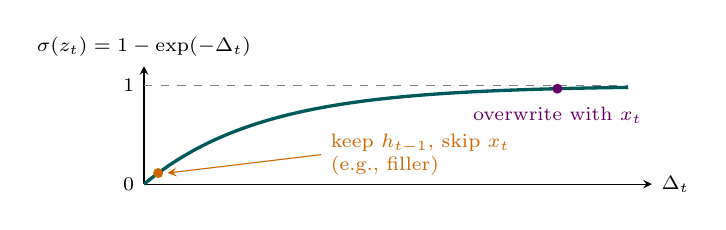
\begin{tikzpicture}[font=\scriptsize]
  \def\xs{1.5} \def\ys{1.25}
  \draw[->, >=stealth] (0, 0) -- ({4.3 * \xs}, 0) node[right] {$\Delta_t$};
  \draw[->, >=stealth] (0, 0) -- (0, {1.2 * \ys}) node[above] {$\sigma(z_t) = 1 - \exp(-\Delta_t)$};
  \draw[gray, dashed] (0, \ys) -- ({4.1 * \xs}, \ys);
  \node[anchor=east] at (0, \ys) {1};
  \node[anchor=east] at (0, 0) {0};
  \draw[teal!70!black, very thick, domain=0:4.1, samples=60] plot ({\x * \xs}, {\ys * (1 - exp(-\x))});
  \fill[orange!80!black] ({0.12 * \xs}, {\ys * (1 - exp(-0.12))}) circle (1.8pt);
  \node[anchor=west, align=left, orange!80!black] (keep) at ({1.5 * \xs}, {0.3 * \ys}) {keep $h_{t-1}$, skip $x_t$\\ (e.g., filler)};
  \draw[->, >=stealth, orange!80!black] (keep.west) -- ({0.2 * \xs}, {\ys * (1 - exp(-0.12))});
  \fill[violet!80!black] ({3.5 * \xs}, {\ys * (1 - exp(-3.5))}) circle (1.8pt);
  \node[anchor=north, align=center, violet!80!black] at ({3.5 * \xs}, {0.88 * \ys}) {overwrite with $x_t$};
\end{tikzpicture}
\end{center}

\vfill

\end{frame}



% ------------------------------------------------------------------------------

% Alternative PAPER FIGURE: Gu and Dao (2024), Figure 1 (selective SSM with
% hardware-aware state expansion)
\begin{frame}{Hardware-Aware Selective Scan}

\vfill

\begin{itemize}
  \item Selection breaks the convolution trick, so we need the scan, over states $N\times$ larger than the input
  \item Naive: write all states $\vec h_t$ to slow GPU memory (HBM)
  \item Mamba fuses discretization, scan, and readout in fast SRAM and writes only $\vec y$
\end{itemize}

\medskip
\medskip


\begin{center}
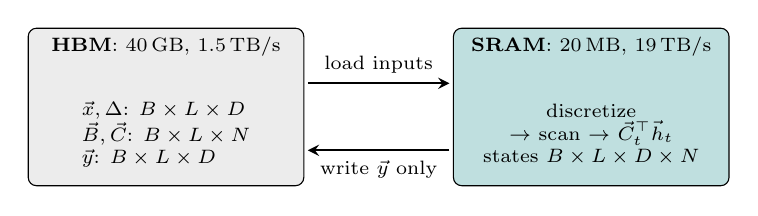
\begin{tikzpicture}[
    font=\scriptsize,
    mem/.style={draw, rounded corners=3pt, minimum width=3.5cm, minimum height=2.0cm},
    flow/.style={->, >=stealth, thick},
  ]
  \node[mem, fill=gray!15] (hbm) at (0, 0) {};
  \node[anchor=north, align=center] at (hbm.north) {\textbf{HBM}: 40\,GB, 1.5\,TB/s};
  \node[align=left] at (0, -0.35) {$\vec x, \Delta$: $B \times L \times D$\\ $\vec B, \vec C$: $B \times L \times N$\\ $\vec y$: $B \times L \times D$};
  \node[mem, fill=teal!25] (sram) at (5.4, 0) {};
  \node[anchor=north, align=center] at (sram.north) {\textbf{SRAM}: 20\,MB, 19\,TB/s};
  \node[align=center] at (5.4, -0.35) {discretize\\ $\rightarrow$ scan $\rightarrow$ $\vec C_t^\top \vec h_t$\\ states $B \times L \times D \times N$};
  \draw[flow] (1.8, 0.3) -- node[above] {load inputs} (3.6, 0.3);
  \draw[flow] (3.6, -0.55) -- node[below] {write $\vec y$ only} (1.8, -0.55);
\end{tikzpicture}
\end{center}

\vfill

\end{frame}


\begin{frame}{Full Mamba Model}
\vfill
\centering
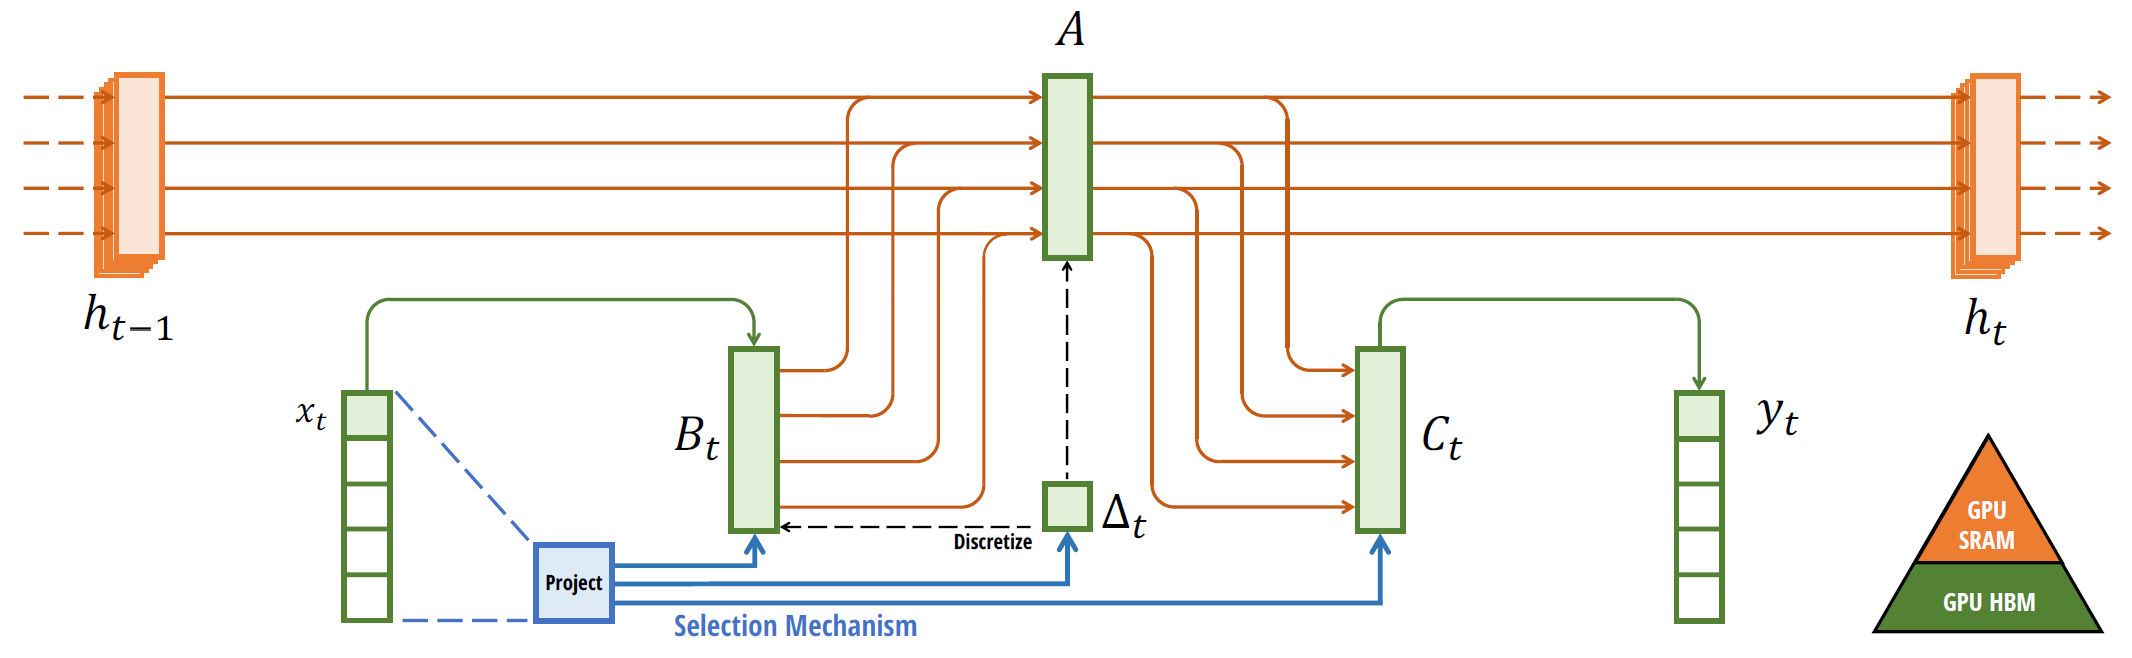
\includegraphics[width=\textwidth]{figure/mamba.png}
\vfill
\end{frame}

% ------------------------------------------------------------------------------



\begin{frame}{Constant-Size State at Inference}

\vfill

\begin{itemize}
  \item Mamba keeps an $N$-dimensional state for each of its $E \cdot D$ channels ($E = 2$: expansion factor), plus last convolution inputs
    \item Mamba-2.8B (64 layers, $D = 2560$): c.\ 6M numbers $\approx$ 12\,MB in 16-bit, for \emph{any} $n$
  \item Transformer of the same size (Pythia-2.8B: 32 layers, $d = 2560$): inference memory grows by 0.33\,MB per token
\end{itemize}

\medskip


\begin{center}
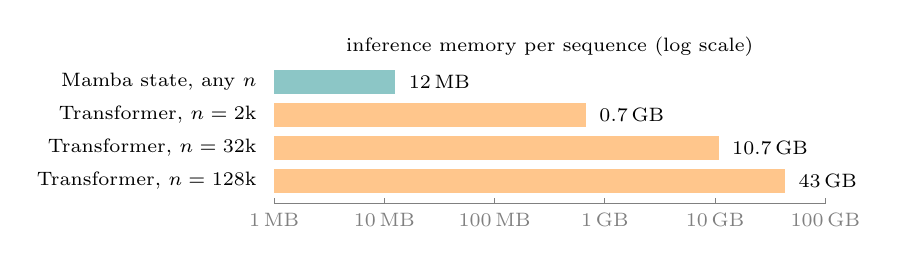
\begin{tikzpicture}[font=\scriptsize]
  \def\sc{1.4}  % cm per decade, axis from 1 MB to 100 GB
  % sizes in MB: 12.5, 671, 10737, 42950; given as log10 (pgfmath overflows above 16383)
  \foreach \lab/\lmb/\txt/\col [count=\r] in {{Mamba state, any $n$}/1.097/{12\,MB}/teal!45,
                                              {Transformer, $n = 2$k}/2.827/{0.7\,GB}/orange!45,
                                              {Transformer, $n = 32$k}/4.031/{10.7\,GB}/orange!45,
                                              {Transformer, $n = 128$k}/4.633/{43\,GB}/orange!45}{
    \pgfmathsetmacro{\y}{-(\r - 1) * 0.42}
    \pgfmathsetmacro{\xx}{\sc * \lmb}
    \fill[\col] (0, \y) rectangle (\xx, \y + 0.3);
    \node[anchor=east] at (-0.1, \y + 0.15) {\lab};
    \node[anchor=west] at (\xx + 0.05, \y + 0.15) {\txt};
  }
  \draw[gray] (0, -1.4) -- ({5 * \sc}, -1.4);
  \foreach \e/\lab in {0/1\,MB, 1/10\,MB, 2/100\,MB, 3/1\,GB, 4/10\,GB, 5/100\,GB}{
    \draw[gray] ({\e * \sc}, -1.4) -- ({\e * \sc}, -1.32);
    \node[anchor=north, gray] at ({\e * \sc}, -1.4) {\lab};
  }
  \node[anchor=south] at ({2.5 * \sc}, 0.35) {inference memory per sequence (log scale)};
\end{tikzpicture}
\end{center}

\vfill

\end{frame}

% ------------------------------------------------------------------------------

% PAPER FIGURES: Gu and Dao (2024), Figure 4 (scaling laws on the Pile) and
% Figure 8 (efficiency: scan vs. FlashAttention-2, inference throughput).
% Save as figure/mamba-scaling.png and figure/mamba-efficiency.png
\begin{frame}{Mamba Performance}

\vfill

\begin{itemize}
  \item Scaling laws on the Pile: first attention-free model to match a strong transformer recipe (Transformer++)
  \item Mamba-3B outperforms transformers of the same size and matches transformers twice its size
  \item $5\times$ higher generation throughput, keeps improving with context up to 1M tokens (DNA, audio)
\end{itemize}

\medskip
\medskip

\centering
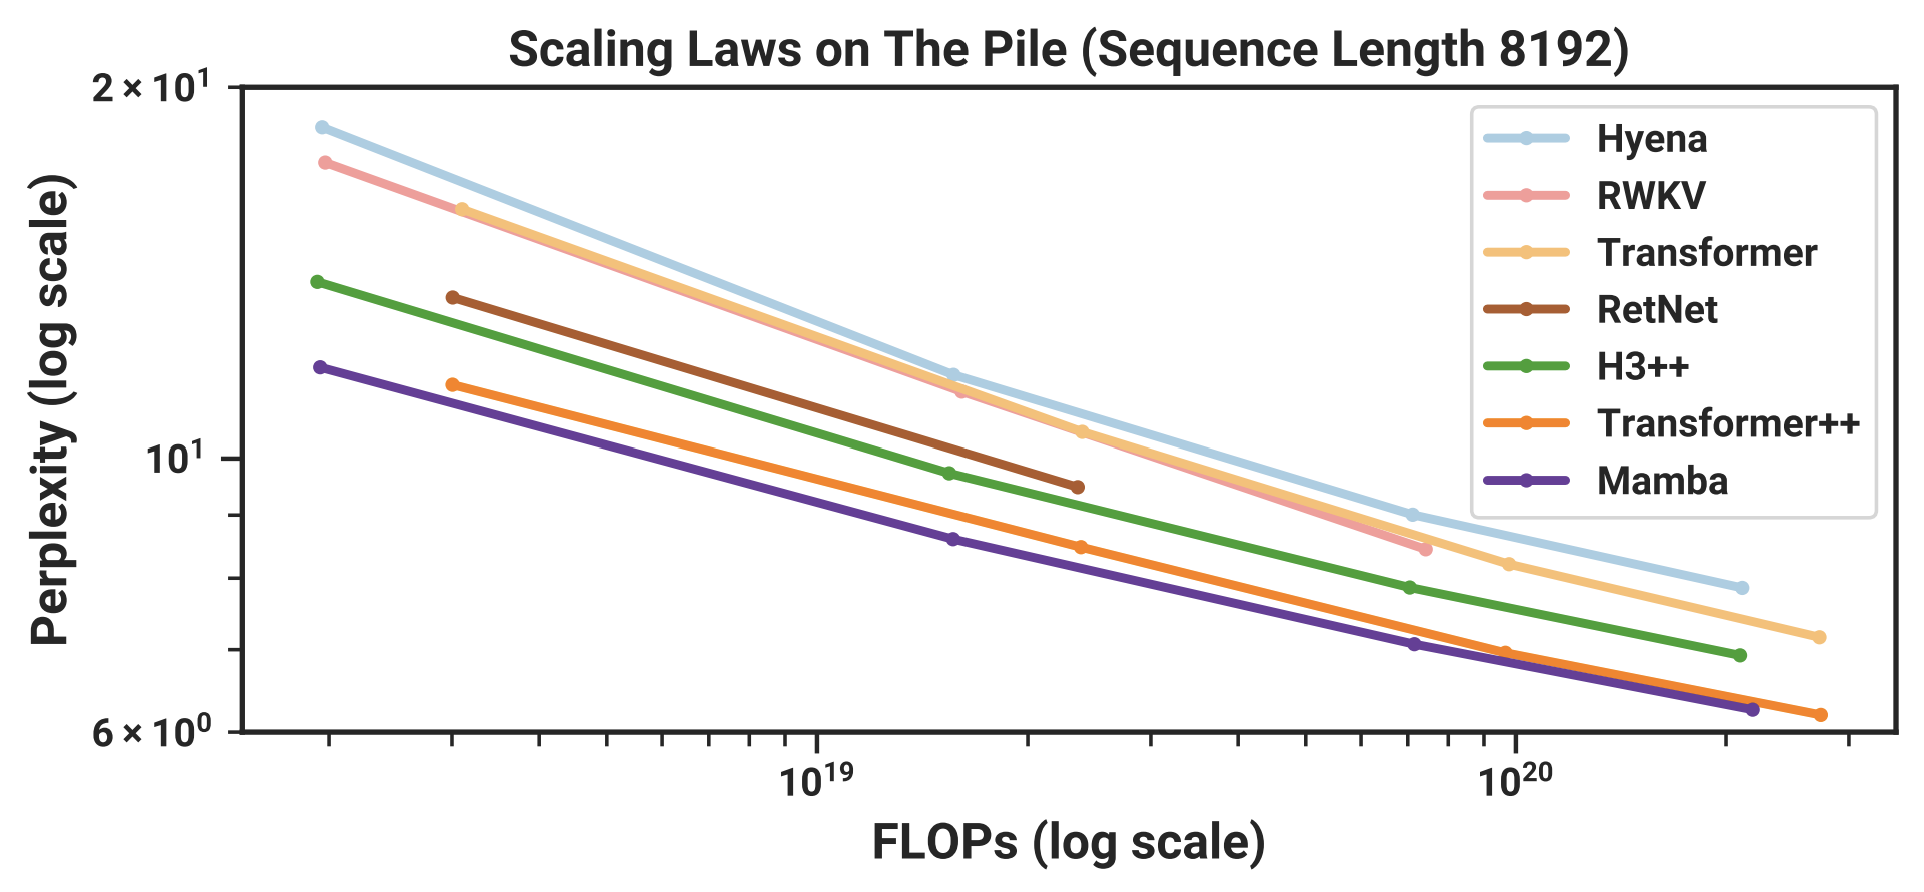
\includegraphics[width=0.7\textwidth]{figure/mamba_perplexity.png}

\vfill

\end{frame}

% ------------------------------------------------------------------------------

% Optional PAPER FIGURE: Jelassi et al. (2024), Figure 1 (copying accuracy vs.
% string length, transformer vs. SSMs)
\begin{frame}{The Limits of a Fixed-Size State}

\vfill

\begin{itemize}
  \item Everything must fit into $\vec h_t$: state is \textbf{lossy} ($\neq$ transformers)
  \item Copying and retrieval suffer: transformers copy much longer strings than SSMs \citebutton{Jelassi et al. (2024) \cite{jelassi2024repeat}}{https://arxiv.org/abs/2402.01032}
  \item 8B scale: pure Mamba(-2) lags on 5-shot MMLU and phonebook lookup, but a hybrid with 7\,\% attention layers beats the transformer \citebutton{Waleffe et al. (2024) \cite{waleffe2024empirical}}{https://arxiv.org/abs/2406.07887}
\end{itemize}

\medskip
\medskip


\begin{center}
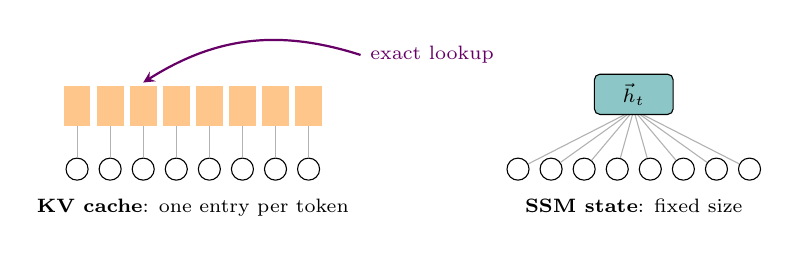
\begin{tikzpicture}[
    font=\scriptsize,
    tok/.style={circle, draw, fill=white, inner sep=0pt, minimum size=2.8mm},
    flow/.style={->, >=stealth},
  ]
  % ---- KV cache --------------------------------------------------------------------------
  \foreach \p in {1,...,8}{
    \node[tok] (t\p) at ({(\p - 1) * 0.42}, 0) {};
    \fill[orange!45] ({(\p - 1) * 0.42 - 0.17}, 0.55) rectangle ++(0.34, 0.5);
    \draw[gray!60] (t\p) -- ({(\p - 1) * 0.42}, 0.55);
  }
  \draw[flow, thick, violet!80!black] (3.6, 1.45) to[bend right=25] ({2 * 0.42}, 1.1);
  \node[anchor=west, violet!80!black] at (3.6, 1.45) {exact lookup};
  \node[anchor=north, align=center] at (1.47, -0.25) {\textbf{KV cache}: one entry per token};
  % ---- SSM state -------------------------------------------------------------------------
  \foreach \p in {1,...,8}{
    \node[tok] (s\p) at ({5.6 + (\p - 1) * 0.42}, 0) {};
    \draw[gray!60] (s\p) -- (7.07, 0.75);
  }
  \node[draw, rounded corners=2pt, fill=teal!45, minimum width=1.0cm, minimum height=5mm] at (7.07, 0.95) {$\vec h_t$};
  \node[anchor=north, align=center] at (7.07, -0.25) {\textbf{SSM state}: fixed size};
\end{tikzpicture}
\end{center}

\vfill

\end{frame}

% ------------------------------------------------------------------------------


% ------------------------------------------------------------------------------

\begin{frame}{Hybrid Models}

\vfill

\begin{itemize}
  \item Many recent long-context LLMs combine \textbf{many} linear-recurrent layers with \textbf{a few} attention layers
  \item Recurrent layers: constant-size state vs.\ attention layers: exact lookup into the past
  \item Recurrent layer of choice: Mamba-2 or gated linear attention with the delta rule (Gated DeltaNet) \citebutton{Yang et al. (2025) \cite{yang2025gated}}{https://arxiv.org/abs/2412.06464}
\end{itemize}

\medskip


\begin{center}
\footnotesize
\setlength{\tabcolsep}{4.5pt}
\begin{tabular}{@{}llrllr@{}}
  \toprule
  Model             & Year & Total & Recurrent layer      & Attention & Ratio \\
  \midrule
  Jamba             & 2024 & 52B   & Mamba                & softmax   & 7\,:\,1 \\
  MiniMax-01        & 2025 & 456B  & lightning attention  & softmax   & 7\,:\,1 \\
  Qwen3-Next        & 2025 & 80B   & Gated DeltaNet       & gated     & 3\,:\,1 \\
  Kimi Linear       & 2025 & 48B   & Kimi Delta Attention & MLA       & 3\,:\,1 \\
  Nemotron 3 Nano   & 2025 & 32B   & Mamba-2              & softmax   & 4\,:\,1 \\
  Qwen3.5           & 2026 & 397B  & Gated DeltaNet       & gated     & 3\,:\,1 \\
  Nemotron 3 Super  & 2026 & 120B  & Mamba-2              & softmax   & 5\,:\,1 \\
  \bottomrule
\end{tabular}
\end{center}

\vfill

\end{frame}

% ------------------------------------------------------------------------------




 
 

\begin{frame}[allowframebreaks,noframenumbering,plain]{References}
\vfill
        \tiny
        \bibliographystyle{plain} %apalike
        \bibliography{refs-ssms}
\vfill
\end{frame}

\endlecture
\end{document}
